% mnras_template.tex
%
% LaTeX template for creating an MNRAS paper
%
% v3.0 released 14 May 2015
% (version numbers match those of mnras.cls)
%
% Copyright (C) Royal Astronomical Society 2015
% Authors:
% Keith T. Smith (Royal Astronomical Society)

% Change log
%
% v3.0 May 2015
%    Renamed to match the new package name
%    Version number matches mnras.cls
%    A few minor tweaks to wording
% v1.0 September 2013
%    Beta testing only - never publicly released
%    First version: a simple (ish) template for creating an MNRAS paper

%%%%%%%%%%%%%%%%%%%%%%%%%%%%%%%%%%%%%%%%%%%%%%%%%%
% Basic setup. Most papers should leave these options alone.
\documentclass[fleqn,usenatbib]{mnras}

% MNRAS is set in Times font. If you don't have this installed (most LaTeX
% installations will be fine) or prefer the old Computer Modern fonts, comment
% out the following line
\usepackage{newtxtext,newtxmath}
% Depending on your LaTeX fonts installation, you might get better results with one of these:
%\usepackage{mathptmx}
%\usepackage{txfonts}

% Use vector fonts, so it zooms properly in on-screen viewing software
% Don't change these lines unless you know what you are doing
\usepackage[T1]{fontenc}
\usepackage{ae,aecompl}
%\usepackage{booktabs}

%%%%% AUTHORS - PLACE YOUR OWN PACKAGES HERE %%%%%

% Only include extra packages if you really need them. Common packages are:
\usepackage{graphicx}	% Including figure files
\usepackage{amsmath}	% Advanced maths commands
%\usepackage{amssymb}	% Extra maths symbols
\usepackage{lscape}

%%%%%%%%%%%%%%%%%%%%%%%%%%%%%%%%%%%%%%%%%%%%%%%%%%

%%%%% AUTHORS - PLACE YOUR OWN COMMANDS HERE %%%%%
%\DeclareUnicodeCharacter{2212}{-}

% Please keep new commands to a minimum, and use \newcommand not \def to avoid
% overwriting existing commands. Example:
%\newcommand{\pcm}{\,cm$^{-2}$}	% per cm-squared

%%%%%%%%%%%%%%%%%%%%%%%%%%%%%%%%%%%%%%%%%%%%%%%%%%

%%%%%%%%%%%%%%%%%%% TITLE PAGE %%%%%%%%%%%%%%%%%%%

% Title of the paper, and the short title which is used in the headers.
% Keep the title short and informative.
\title[GPM for Faraday Depth Spectra]{Gaussian Process Modeling to Recover Faraday Depth Spectra}

% The list of authors, and the short list which is used in the headers.
% If you need two or more lines of authors, add an extra line using \newauthor
\author[S.~W.~Ndiritu et al.]{
S.~W.~Ndiritu,$^{1,2}$\thanks{E-mail: sndiritu@mpa-garching.mpg.de
 (SWN)}
A.~M.~M.~Scaife$^{2,3}$,
D.~Tabb$^{4}$,
M.~C{\'a}rcamo$^{2,5}$ \&
J.~Hanson$^{2}$ \\
% List of institutions
$^{1}$ Max Planck Institute for Astrophysics, Karl-Schwarzschildstra{\ss}e 1, 85748 Garching, Germany \\
$^{2}$ Jodrell Bank Centre for Astrophysics, School of Physics and Astronomy, University of Manchester, Alan Turing Building,\\ Oxford Road, Manchester, M13 9PL, UK \\
$^{3}$ The Alan Turing Institute, Euston Road, London NW1 2DB, UK \\
$^{4}$ Stellenbosch University, Stellenbosch Central, Stellenbosch, South Africa \\
$^{5}$ Departamento de Ingenier\'ia Inform\'atica, Universidad de Santiago de Chile, Av. Ecuador 3659, Santiago, Chile \\
}

% These dates will be filled out by the publisher
\date{Accepted XXX. Received YYY; in original form ZZZ}

% Enter the current year, for the copyright statements etc.
\pubyear{2019}

% Don't change these lines
\begin{document}
\label{firstpage}
\pagerange{\pageref{firstpage}--\pageref{lastpage}}
\maketitle

% Abstract of the paper
\begin{abstract}
The presence of missing data in complex polarization measurements from radio telescopes negatively affects both the rotation measure (RM) transfer function and the Faraday depth spectra derived from these data. Such gaps in polarization data are mostly caused by flagging of radio frequency interference and their effects worsen as the percentage of missing data increases. In this paper we present a novel method for reconstructing missing polarization data based on Gaussian processes (GPs). Gaussian processes are stochastic processes that enable us to encode prior knowledge in our models. They also provide a comprehensive way of incorporating and quantifying uncertainties in regression modelling. In addition to imputing missing values, we also demonstrate that Gaussian process modelling can be used for recovering rotation measure values directly from complex polarization data, and that reconstructing missing polarization data using this probabilistic method improves the appearance and the resolution of the Faraday depth spectra.
\end{abstract}

% Select between one and six entries from the list of approved keywords.
% Don't make up new ones.
\begin{keywords}
techniques: polarimetric -- methods: statistical -- radio continuum: general
\end{keywords}

%%%%%%%%%%%%%%%%%%%%%%%%%%%%%%%%%%%%%%%%%%%%%%%%%%

%%%%%%%%%%%%%%%%% BODY OF PAPER %%%%%%%%%%%%%%%%%%

\section{Introduction}

Polarisation measurements from radio telescopes with broadband receiver systems have changed the way in which we investigate magnetised astrophysical plasmas by enabling the use of the RM synthesis method \citep{1966MNRAS.133...67B, 2005A&A...441.1217B}. In this method the Fourier relationship between polarized intensity as a function of wavelength-squared and the Faraday dispersion function is exploited to recover the polarized intensity as a function of Faraday depth, $\phi$, such that
%
\begin{equation}
\label{eq:fourier}
F(\phi) = \int_{-\infty}^{\infty}{ P(\lambda^2){\rm e}^{-2i\phi \lambda^2}~{\rm d}\lambda^2 },
\end{equation}
%
where
%
\begin{equation}
\label{eq:pol}
P(\lambda^2) = |P(\lambda^2)|{\rm e}^{2i\chi(\lambda^2)} = Q(\lambda^2) + iU(\lambda^2).
\end{equation}

Although conceptually simple, in practical terms the implementation of this method and the interpretation of the resulting Faraday dispersion function are complicated by a number of factors. The first of these complications is that the Stokes pseudo-vectors $Q$ and $U$ are not sampled natively in wavelength-squared but linearly in frequency. A further complication is that Eq.~\ref{eq:fourier} does not represent a true Fourier relationship as $P(\lambda^2)$ does not exist at $\lambda^2 < 0$. Since $F(\phi)$ is not necessarily a purely real quantity this represents a fundamental limitation in attempting to reconstruct an unknown Faraday dispersion function from measured values of $P(\lambda^2)$. An additional limitation comes from the finite bandwidth and hence range of wavelength-squared, $\Delta (\lambda^2)$, measured by a radio telescope receiver, as well as the potentially incomplete sampling over this bandwidth due to various effects (RFI, instrumental problems etc.) that require flagging (excision) of specific frequency channel data during an observation.

In order to exploit the use of Fast Fourier Transforms (FFTs), computational approaches to RM Synthesis employ an initial processing step to re-bin spectral data, $Q(\nu)~\&~U(\nu)$, into regularly spaced arrays of $\lambda^2$. This approach produces regularly sampled data arrays, $Q(\lambda^2)~\&~U(\lambda^2)$ that are multiplied by a weighting function, $W(\lambda^2)$, which is non-zero where measurements are present but which will also contain a (potentially significant) number of zero-valued elements due to the non-linear mapping of $\nu$ to $\lambda^2$. This  multiplication results in the convolution of the Faraday dispersion function with a transfer function,
%
\begin{equation}
\label{eq:rmtf}
{\rm RMTF}(\phi) = \frac{\int_{-\infty}^{\infty} { W(\lambda^2){\rm e}^{-2i\phi\lambda^2}~{\rm d}\lambda^2 }}{\int_{-\infty}^{\infty} { W(\lambda^2)~{\rm d}\lambda^2 }},
\end{equation}
%
known as the rotation measure transfer function, RMTF$(\phi)$. Consequently, the complications caused by both the $\lambda^2 < 0$ problem and the mapping of linear frequency to wavelength-squared may be encapsulated in the weighting function $W(\lambda^2)$ and its Fourier counterpart, RMTF($\phi$). Although attempts have been made to deconvolve the RMTF from the Faraday depth spectra, e.g. \cite{2009IAUS..259..591H}, the  methods are inherently underconstrained due to the $P(\lambda^2<0) = \varnothing$ problem, resulting in a statistical ambiguity in the results.

These issues are of particular importance when complex or compound Faraday structures are seen along a single line of sight. In a blind data challenge comparing different methods for extracting the parameters of Faraday structures, \cite{Sun_2015} noted that RM synthesis was highly prone to missing composite Faraday structures and that the $\sim$25\% of extragalactic sources seen observationally to have such structures \citep{law2011} was likely to be an underestimate. \cite{Sun_2015} concluded that when Faraday complexity is present, only QU-fitting methods will produce results that do not introduce extraneous scatter in recovered RM values. Such QU-fitting methods, e.g. \cite{Farnsworth_2011, 10.1111/j.1365-2966.2012.20554.x, 2014ApJ...792...51I}, model the observed polarization, $\tilde{P}(\lambda^2)$, directly rather than decomposing Faraday depth spectra to recover parameters. However, whilst QU-fitting methods can be more reliable for recovering composite structures, in particular those including Faraday thick components, they rely on physically parametrised models of the synchrotron-emitting and Faraday rotating media along the line of sight to be known a priori.

In this work we explore the potential for using a Gaussian Process Modelling (GPM) approach to improve both the interpretation of Faraday depth spectra and the recovery of physical parameters from polarization measurements. In its simplest form, a GPM approach can be considered part of the family of QU-fitting methods; however, it has certain advantages over physically parameterised model-fitting methods, which include both a robustness to using non-exact models for imperfectly known datasets and an ability to provide predictive models for imputation including posterior variances.  The contents of this paper are as follows, in \S~\ref{sec:method} we describe the underlying GPM methodology including a description of the covariance kernel function employed and the optimization of hyper-parameters; in \S~\ref{sec:sims} we illustrate the impact of GP optimisation and re-sampling of polarization data on their resulting Faraday depth spectra in the presence of significant RFI flagging, and demonstrate how the rotation measures for Faraday thin data can be recovered from the hyper-parameters of the GP; in \S~\ref{sec:joedata} we demonstrate the method using a simulated source population with observational specifications matching that of the MeerKAT radio telescope; in \S~\ref{sec:disc} we discuss the implications of these results, compare the method to previous work in the literature and consider the use of more complex covariance kernels. In Section~\ref{sec:conclusions} we draw our conclusions.

\section{Gaussian Process Modelling for Faraday Depth Reconstruction}
\label{sec:astrogpm}

Gaussian Processes (GPs) are probabilistic non-parametric models that can be used for a variety of regression and classification problems. A Gaussian Process Model (GPM) can be used to describe a given dataset by assuming a priori that the data themselves represent a realisation of a stochastic process described by a multi-variate Gaussian distribution. Such models are non-parametric as the Gaussian process (GP) is a prior on the data itself rather than on a parametric model, i.e. the complexity of the model grows with the inclusion of additional data points. GPMs are considered to be an attractive solution when modelling systems where the degree of complexity required by a parametric model is not necessarily supported by the amount of information in the observations. Overly complex parametric models are prone to over-fitting and can lead to misinterpretation of the data. In contrast, Gaussian processes are flexible probabilistic regression models that do not require exact knowledge of the underlying physical model and can also provide posterior uncertainties that naturally reflect high uncertainty in regions of data space where there are few observational constraints.

In astrophysics, Gaussian processes have been used in various applications including in the study of photometric redshifts \citep{wa06300n}, variability in stellar light curves \citep{2018MNRAS.474.2094A}, Galactic dust emission \citep{ensslinfromert}, eclipses in cataclysmic variable stars \citep{10.1093/mnras/stw2417}, transmission spectroscopy of extrasolar planets \citep{2012MNRAS.419.2683G}, and radio velocity studies for planetary candidates \citep{10.1093/mnras/stv1428}. It has also been used extensively in cosmic microwave background analysis \citep{1987MNRAS.226..655B, 1999CoScE...1...21B, PhysRevD.67.023001}, as well as for modelling instrumental systematics and calibration, e.g. \cite{2012MNRAS.419.2683G, 2014MNRAS.443.2517H, 2015ApJ...800...46B, Czekala_2015, 2015MNRAS.451..680E, 10.1093/mnras/stv1428, 2015Natur.526..546V, 2016MNRAS.459.2408A, 2016MNRAS.456L...6R, 2017MNRAS.466.4250L}.

\subsection{GPM for imputation of missing polarization data}
\label{sec:imputation}

The transfer function described in Equation~\ref{eq:rmtf} is a function of the observational sampling in $\lambda^2$-space. In practice this sampling is affected not only by the characteristics of the telescope's receiver system but also by the necessary removal of frequency channels affected by radio frequency interference (RFI). Radio telescopes operating at or close to L-band (1.4\,GHz) typically experience data flagging at a level of $20-50\%$ in bandwidth due to a wide variety of both terrestrial and satellite RFI sources [REF]. As well as negatively impacting the sensitivity of an observation, this flagging can also result in large contiguous gaps in the frequency coverage that have a detrimental effect on the form of the RMTF.

Contingent on there being sufficient information in the remaining data, Gaussian process modelling may provide a potential method for reconstructing these missing data subject to only weak assumptions about the form of the data and without the need for a parameterised physical model. Furthermore, GPM not only provides a prediction of the value for each missing data point but also an uncertainty on that value, allowing astronomers to set thresholds on the degree of reliability they are prepared to accept when imputing the values of missing data points.

\subsection{GPM for resampling of irregular data}
\label{sec:resampling}

In addition to the imputation of missing data values, GPM can also provide a method of re-sampling observational data onto a uniformly spaced $\lambda^2$-space. Since data are natively taken in channels uniformly space in frequency, practical implementations of RM Synthesis require these data to be re-sampled, or {\it gridded}, into a regularly spaced array of $\lambda^2$-positions in order to use an FFT transformation into Faraday depth space, as implemented in for example {\sc pyrmsynth}\footnote{\url{https://github.com/mrbell/pyrmsynth}} package that was used to perform RM synthesis for the LOFAR Two-metre Sky Survey \citep{lofarpyrmsynth}. Like RFI flagging, the non-linear relationship between frequency and wavelength-squared results in a distribution of measured data points that are often separated by large contiguous gaps in $\lambda^2$-space, resulting in high sidelobes in the RMTF. Furthermore, GPM can not only be used to re-sample data within the observed bandwidth but also to predict data beyond the boundaries of that bandwidth. Without additional data, these predictions will be subject to rapidly increasing degrees of uncertainty but may still be used over moderate distances in frequency space to improve the resolution of a measurement in Faraday depth. In practice, re-sampling to uniformly spaced $\lambda^2$-positions and imputing the values of data that are missing due to RFI flagging can be done simultaneously.


\section{Method}
\label{sec:method}

The basic premise of GPM is that, instead of employing a physically motivated or semi-empirical parametric model to describe a dataset, we can instead assume that the data, $y(x)$, represent the realization of a random Gaussian process,
%
\begin{equation}
y(x) = N(\mu(x), K(x,x)),
\end{equation}
%
where $K(x,x)$ is the matrix that defines the degree of covariance between every pair of measurement positions, $(x,x')$, and $\mu(x)$ is an underlying mean function, which in this case is considered to be zero-valued. In the case of non-negligible polarization leakage, this would manifest as $\mu(x)\neq 0$.

The expected value of the data at all other positions, $x_{\ast}$, can be calculated as a posterior mean, $\mu_{\ast}$, with an associated posterior variance, $C_{\ast}$, such that
%
\begin{eqnarray}
\label{eq:postmu} \mu_{\ast} &=&  K(x_{\ast},x)^T K(x,x)^{-1} y  \\
\label{eq:postcov} C_{\ast} &=&  K(x_{\ast},x_{\ast}) - K(x_{\ast},x)^T K(x,x)^{-1} K(x_{\ast},x)
\end{eqnarray}
%
see e.g. \cite{3569, article}.

For polarization data measured at regular intervals in frequency (spectral channels) and hence irregular intervals in $\lambda^2$, the posterior mean can be used to predict the values of the polarization data at regular intervals, $\lambda_{\ast}^2$, avoiding the need for explicit re-binning of the data, and the posterior variance can be used to define the weighting function $W(\lambda_{\ast}^2)$ at those positions and hence calculate the RMTF.

\subsection{Kernel Definition}

The covariance matrix used in Eqs.~\ref{eq:postmu}~\&~\ref{eq:postcov} can be populated analytically using a kernel function, $k$, that defines the degree of covariance for each measurement separation,

\begin{equation}
K(x,x) = \left(
\begin{array}{cccc}
k(x_1,x_1) & k(x_1,x_2) & ... & k(x_1,x_n) \\
k(x_2,x_1) & k(x_2,x_2) & ... & k(x_2,x_n) \\
\vdots & \vdots & \vdots & \vdots \\
k(x_n,x_1) & k(x_n,x_2) & ... & k(x_n,x_n)
\end{array}
\right),
\end{equation}
%
where $k(x_1,x_2)$ is the covariance between two measurements at a separation $|x_1 - x_2|$.

%For complex-valued polarization measurements, each element $k_{ij} = k(x_i, x_j)$ is a $2 \times 2$ matrix, where
%
%\begin{equation}
%k_{ij} = k(x_i, x_j) = \begin{bmatrix} k_{\rm QQ}(x_i,x_j) & k_{\rm QU}(x_i,x_j) \\ k_{\rm UQ}(x_i,x_j) & k_{\rm UU}(x_i,x_j) \end{bmatrix}.
%\end{equation}
%


\subsection{Covariance kernel definition}
\label{sec:kernels}

For the application to radio polarization data we use a compound covariance kernel. The contributions to this kernel comprise covariance arising both from the expected signal and from the properties of the measurement data. Faraday rotation results in periodicity of the complex polarization signal but the presence of additional Faraday components, including thick structures, can cause deviations from exact periodicity in the data. To represent this behaviour we use a quasi-periodic kernel formed from the multiplication of a exponential kernel and a periodic kernel.

We implement our kernel using the {\tt celerite} Gaussian processing library \citep{celerite}. Traditional GPM scales as $\mathcal{O}(N^3)$. This is due to the need to invert the covariance matrix and often makes GPM computationally intractable for large datasets. In contrast,  the {\tt celerite} GP implementation uses a restricted set of kernels that allow for fast separable evaluation with a linear complexity of $\mathcal{O}(N)$.

The {\tt celerite} kernel has a generalised exponential form,
%
\begin{equation}
    k(x_i,x_j) = \sum_{n=1}^{J}{\alpha_n {\rm e}^{-\beta_n |x_i - x_j|} + \alpha_n^{\ast} {\rm e}^{-\beta_n^{\ast} |x_i - x_j|}},
\end{equation}
%
which can be used to produce a quasi-periodic kernel of the form,
%
\begin{equation}
\label{eq:celkernel}
k_1(x_i,x_j)=h\,{\rm e}^{-c|x_i - x_j|}\left[\cos\left(\frac{2\pi|x_i - x_j|}{P}\right)\right].
\end{equation}
%
In this work we combine this quasi-periodic kernel with a white noise kernel,
%
\begin{equation}
\label{eq:whitekernel}
k_2(x_i,x_j)=\sigma_{\rm n}^2\,\delta_{ij},
\end{equation}
%
to take account of the thermal noise present on observational measurements of the complex polarization. Together, $k_1$ and $k_2$ are used to create a composite kernel
%
\begin{equation}
k = k_1 + k_2,
\end{equation}
%
where the contributions of the different components are governed by the values of their hyper-parameters, $h$, $c$, $P$ and $\sigma^2$.

\subsection{Hyper-parameter Estimation}
\label{sec:parms}

The values of the hyper-parameters can be optimized by evaluation of a likelihood function using the measured data. Polarization data are complex valued,
%
\begin{equation}
P(\nu) = Q(\nu) + iU(\nu)
\end{equation}
%
and so the loglikelihood function can be broken down,
%
\begin{equation}
\label{eq:loglike}
\log L = \log L_{\rm Q} + \log L_{\rm U}
\end{equation}
%
The components of this likelihood are
%
\begin{eqnarray}
\log L_{\rm Q} &=& -\frac{1}{2}(Q - \mu_{\rm Q})^{\rm T}K_{\rm Q}^{-1}(Q - \mu_{\rm Q}) - \frac{1}{2}\ln |K_{\rm Q}|\\
\log L_{\rm U} &=& -\frac{1}{2}(U - \mu_{\rm U})^{\rm T}K_{\rm U}^{-1}(U - \mu_{\rm U}) - \frac{1}{2}\ln |K_{\rm U}|
\end{eqnarray}
%
where,
%
\begin{eqnarray}
\mu_{Q} &=& K_{\rm Q}(x_{\ast},x)^T K_{\rm Q}(x,x)^{-1} Q\\
\mu_{U} &=& K_{\rm U}(x_{\ast},x)^T K_{\rm U}(x,x)^{-1} U.
\end{eqnarray}
%
In the case where the covariance matrix is characterised solely by stationary kernels, i.e. kernels that are functions of the sample separation, $|x_i - x_j|$, only, it can be assumed that $K_{\rm U}\equiv K_{\rm Q}$ and in this paper we assume a single kernel of the form given in Equation~\ref{eq:celkernel} to describe both Stokes parameters, the hyper-parameters of which are optimised using the joint likelihood in Equation~\ref{eq:loglike}.

%\subsection{Re-sampling Definition}
%\label{sec:resamp}

%There are two aspects that can be addressed through resampling. The first is the regularity of measurements in $\lambda^2$-space. This regularity reduces the effect of the transfer function in Faraday depth and lowers the contamination from the RMTF side-lobes. The second effect is to increase the accessible range of $\lambda^2$-space. This can be achieved by extending the maximum and minimum limits in $\lambda^2$-space.

%To re-sample onto a regular grid in $\lambda^2$-space we need to set a step size $(\delta \lambda_{\ast}^2)$ as our regular interval. The step size that we choose will determine the maximum Faraday depth to which we have sensitivity. We can therefore chose a step size based on our desired range of Faraday depths. In practice the data will normally allow for higher maximum values than are required as astrophysical Faraday depths are typically small due to the correspondingly low electron densities and magnetic field strengths, even in the presence of very large path lengths. For Galactic fields, Faraday depths are normally limited to a range of $\pm10$\,rad\,m$^{-2}$, for external galaxies they are in the range $\sim100$\,rad\,m$^{-2}$ and for galaxy clusters typically $<1000$\,rad\,m$^{-2}$. With the exception of a few rare cases, there is no need to sample $\lambda^2$ more finely than corresponds to these values, such that,
%
%\begin{equation}
% \delta (\lambda^2) = \frac{\sqrt{3}}{||\phi_{\rm max}||}.
%\end{equation}
%
%In what follows we specify a maximum Faraday depth of 500\,rad\,m$^{-2}$.

%To extend the bandwidth $\Delta \lambda^2$, we apply the same approach and discard the five largest separations in the measured data. We then adopt the sixth largest separation as an extension in $\lambda^2$-space. This is represented graphically in Figure~\ref{fig:resampling}. The effect of this increase in available $\Delta \lambda^2$ is to improve the resolution somewhat in Faraday depth space,
%
%\begin{equation}
%\delta \phi = \frac{2\sqrt{3}}{\Delta (\lambda^2)},
%\end{equation}
%
%and to increase the sensitivity to extended Faraday structures,
%
%\begin{equation}
%\label{eq:fdscale}
%\Delta \phi = \frac{\pi}{\lambda_{\rm min}^2}.
%\end{equation}

\begin{figure}
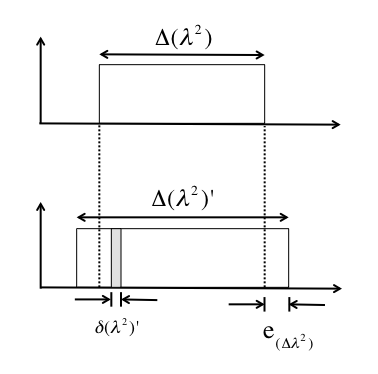
\includegraphics[width=0.5\textwidth]{./FIGURES/faraday_resampling.png}
\caption{\label{fig:resampling} Illustration of the different parameters used to characterise the original input data (top) and the reconstructed data from the optimised GP model (bottom).}
\end{figure}

\section{Application to Simulated Data}
\label{sec:sims}

\subsection{Example scenarios}
\label{sec:scenarios}

We illustrate the use of the GPM method on two examples: (1) a simple Faraday Thin scenario, and (2) a more complex scenario involving both Faraday Thin and Faraday Thick components. This second scenario corresponds to the example geometry outlined in \S~1 of \cite{2005A&A...441.1217B}.

\vskip .1in
\noindent
\textbf{Scenario One} In this scenario we assume polarized emission from the lobe of a radio galaxy with an intensity of 1\,Jy at a reference frequency of $\nu_{\rm ref} = 1.4$\,GHz and a synchrotron spectral index of $\alpha = 0.7$, which has a single valued Faraday depth of 50\,rad\,m$^{-2}$ such that,
%
\begin{eqnarray}
P_{\rm rg}(\lambda^2) &=&  \left(\frac{\lambda^2}{\lambda_{\rm ref}^2}\right)^{\alpha/2}\exp (2i\phi_1 \lambda^2) \\
&=&  \left(\frac{\lambda^2}{\lambda^2_{\rm ref}}\right)^{\alpha/2} \left[\cos (2\phi_1 \lambda^2) +  i \sin (2\phi_1 \lambda^2)\right].
\end{eqnarray}

\vskip .1in
\noindent
\textbf{Scenario Two} In this scenario we adopt the line of sight geometry of \cite{2005A&A...441.1217B}.

\begin{equation}
F_{\rm gal}(\phi) = \begin{cases}
(2\phi_{\rm fg})^{-1} & -\phi_{\rm fg}~<~\phi~<~\phi_{\rm fg} \\
0 & {\rm elsewhere}
\end{cases}
\end{equation}

\begin{equation}
P_{\rm gal}(\lambda^2) = \frac{\sin (2\phi_{\rm fg} \lambda^2)}{2\phi_{\rm fg}\lambda^2}
\end{equation}
%
and the total polarization is given by
%
\begin{equation}
P_{\rm tot}(\lambda^2) = P_{\rm gal}(\lambda^2) + P_{\rm rg}(\lambda^2)
\end{equation}

In both scenarios we assume that the signal is measured over a frequency bandwidth from 0.58\,GHz to 2.50\,GHz in 512 evenly spaced frequency channels. We map each channel frequency to a corresponding value of $\lambda^2$. For each measurement we assume that $(Q, U, \sigma_{\rm Q}, \sigma_{\rm U})$ are recorded, where $Q$ corresponds to the real part of the polarization and $U$ corresponds to the imaginary component.

\subsection{Faraday Depth Spectra}
\label{sec:fdspectra}

%
\begin{figure*}
\centerline{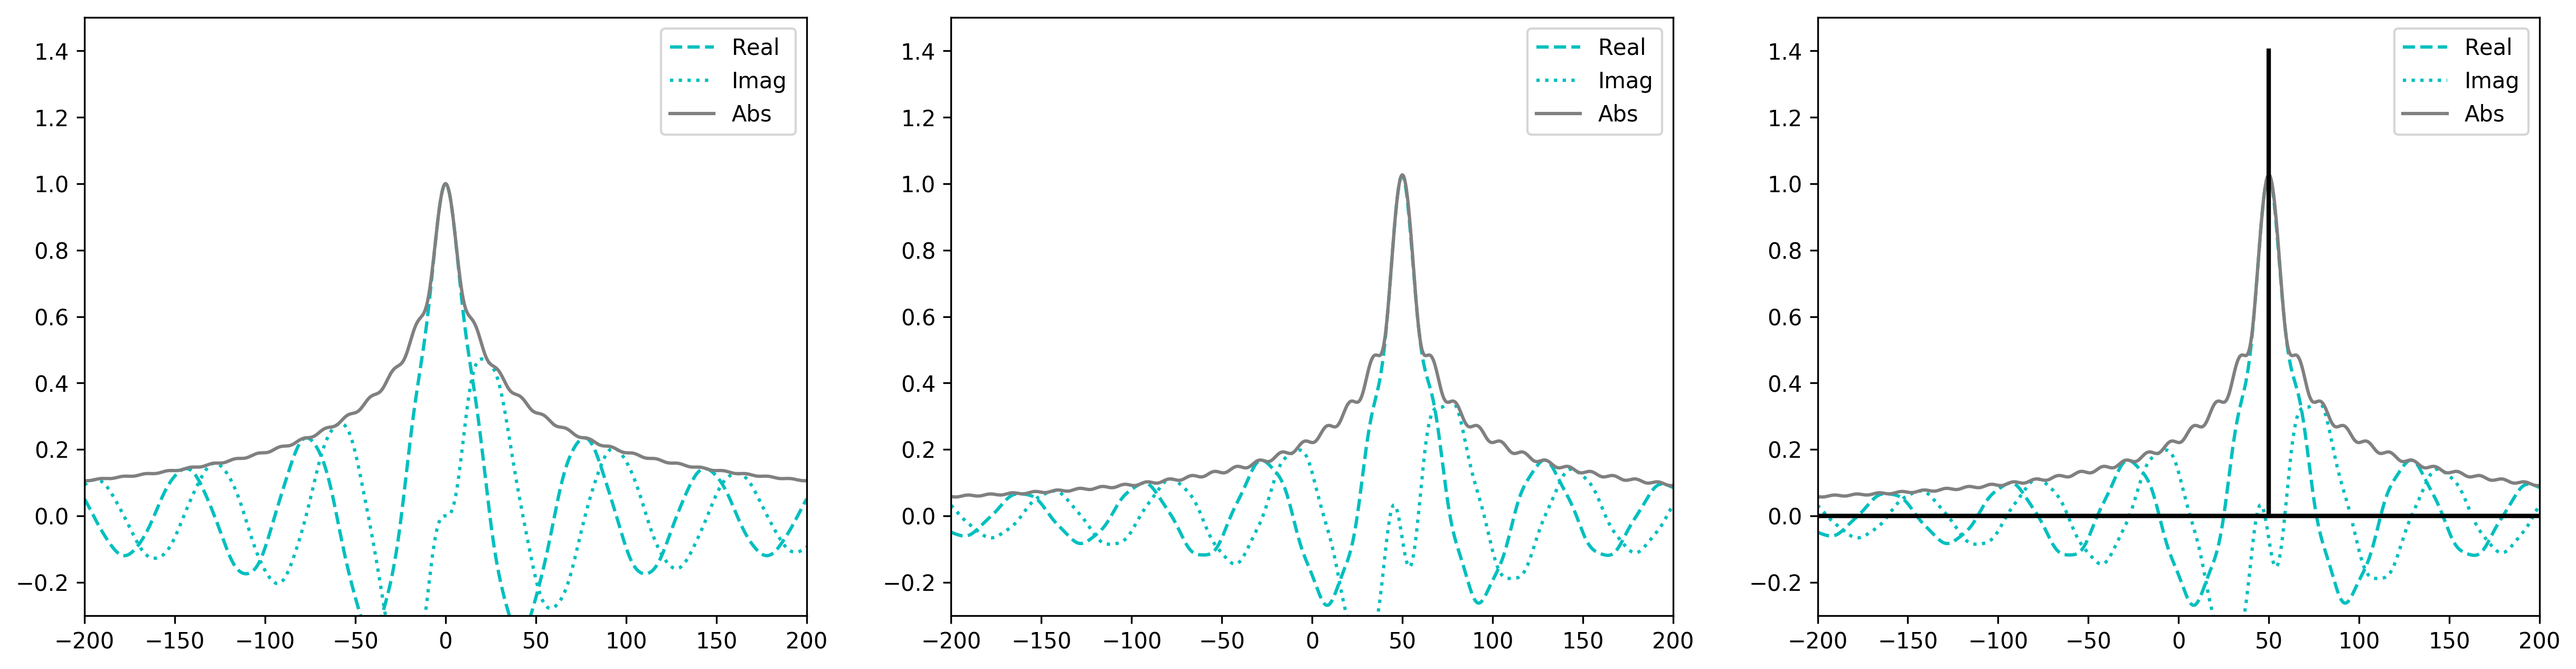
\includegraphics[width=0.9\textwidth]{./FIGURES/Scenario1_fsamp.png}}
\centerline{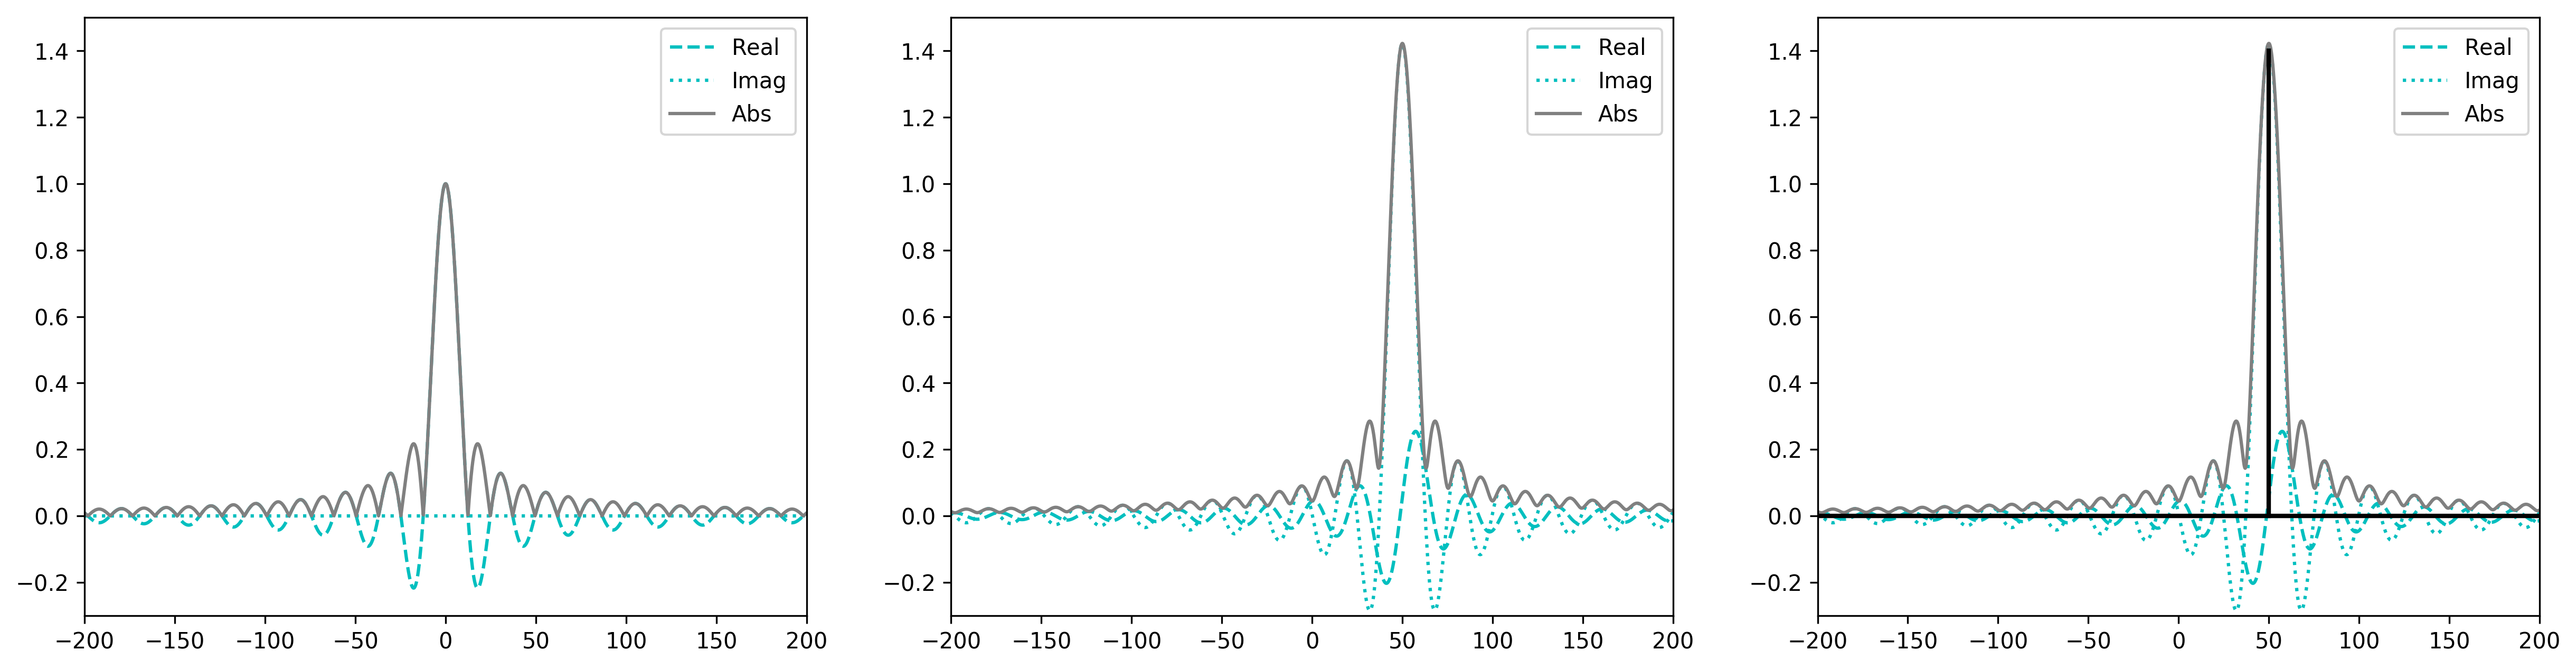
\includegraphics[width=0.9\textwidth]{./FIGURES/Scenario1_lsamp.png}}
\caption{\label{fig:scen1samp} Scenario 1: RMTF (left), Faraday depth spectrum (centre) and Faraday depth spectrum overlaid with input model (right) for the case of (i) data evenly sampled in frequency (top) and (ii) data evenly sampled in wavelength-squared (bottom). Data are noiseless in both cases.}
\end{figure*}
%
We construct Faraday depth spectra for each set of complex polarization data following the numerical method outlined in \cite{2005A&A...441.1217B}. The Faraday depth spectra are calculated using,
%
\begin{equation}
F(\phi) = K^{-1}\sum_{i = 1}^{N}{W_i P_i {\rm e}^{-2j (\lambda_i^2 - \lambda_0^2) \phi}},
\end{equation}
%
where $W_i$ is the weight for channel $i$ at a wavelength of $\lambda_i$, and $P_i$ is the complex polarization measured in that channel, see Equation~\ref{eq:pol}. Correspondingly, the RMTF is calculated using,
%
\begin{equation}
R(\phi) = K^{-1}\sum_{i = 1}^{N}{W_i {\rm e}^{-2j (\lambda_i^2 - \lambda_0^2) \phi}}.
\end{equation}
%
In each case, $K$, is the sum of the weights,
%
\begin{equation}
K = \sum_{i = 1}^{N}{W_i},
\end{equation}
%
where the weights are defined as the reciprocal of the variance in each channel, and $\lambda_0$ is a reference wavelength used to derotate the polarization data to a common zero-point defined as
%
\begin{equation}
\lambda_0^2 = K^{-1}\sum_{i = 1}^{N}{W_i \lambda_i^2}.
\end{equation}

The recovered Faraday depth spectra for Scenario~1 \& Scenario~2 are shown in Figures~\ref{fig:scen1samp}~\&~\ref{fig:scen2samp}, which illustrate the difference in the Faraday depth spectra when polarization data are sampled uniformly in frequency compared to being sampled uniformly in $\lambda^2$-space.
%
\begin{figure*}
\centerline{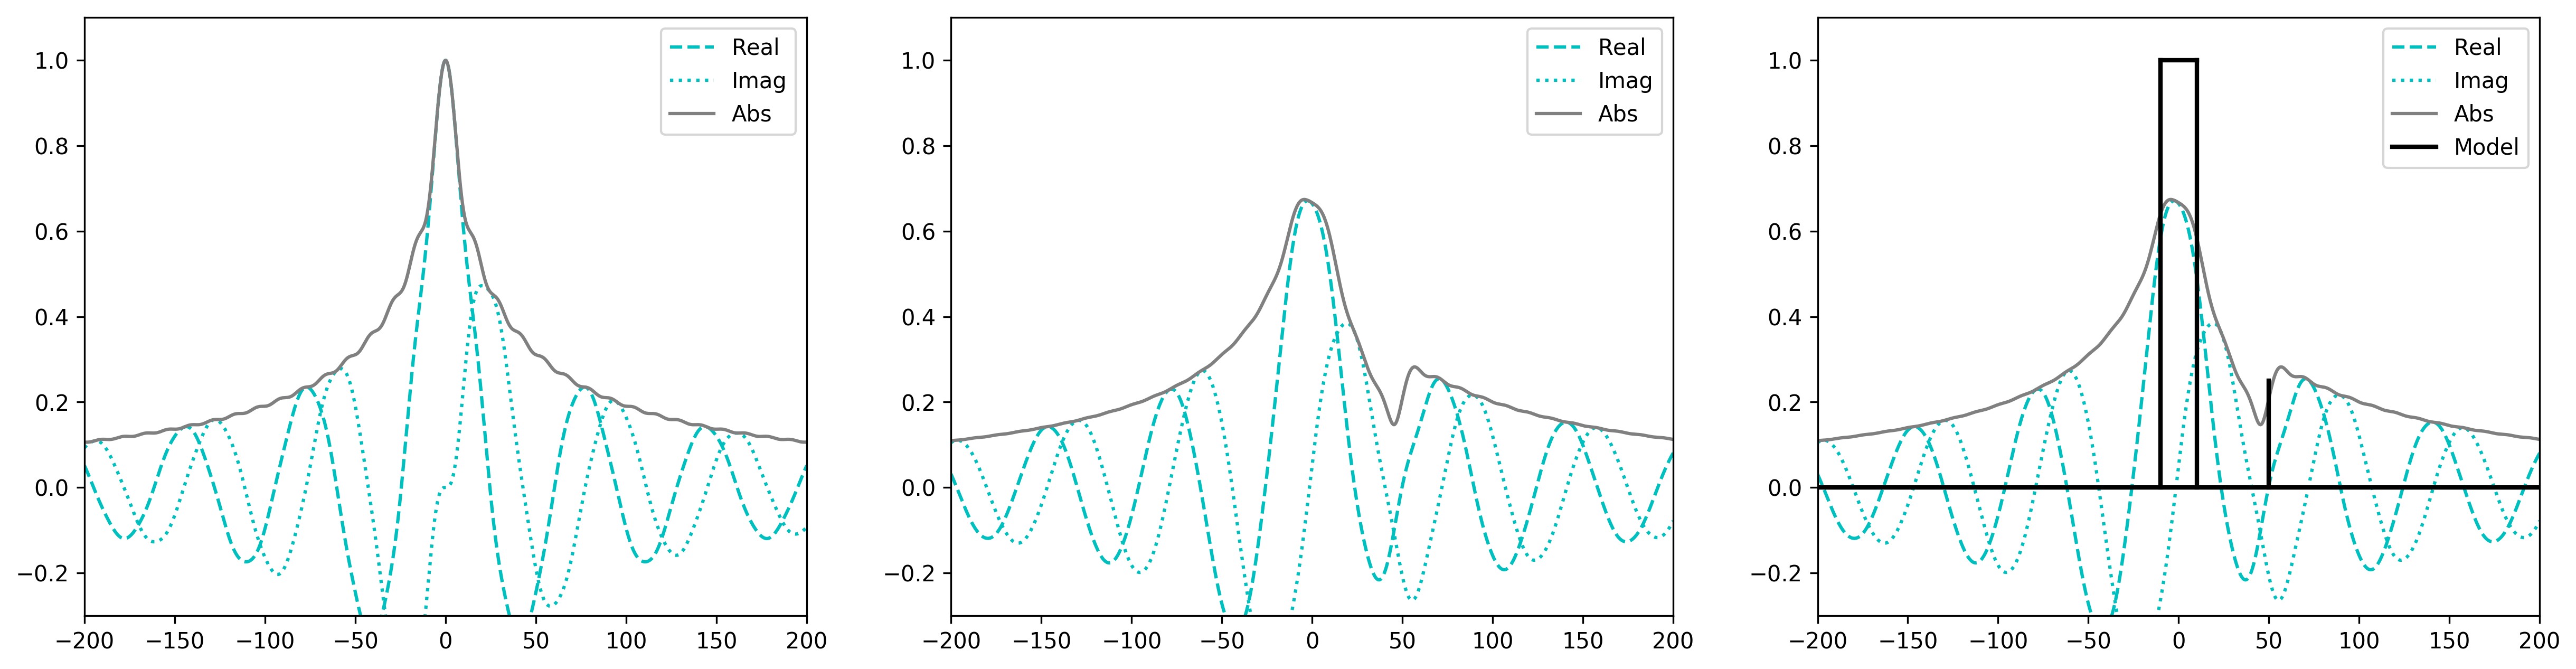
\includegraphics[width=0.9\textwidth]{./FIGURES/Scenario2_fsamp.png}}
\centerline{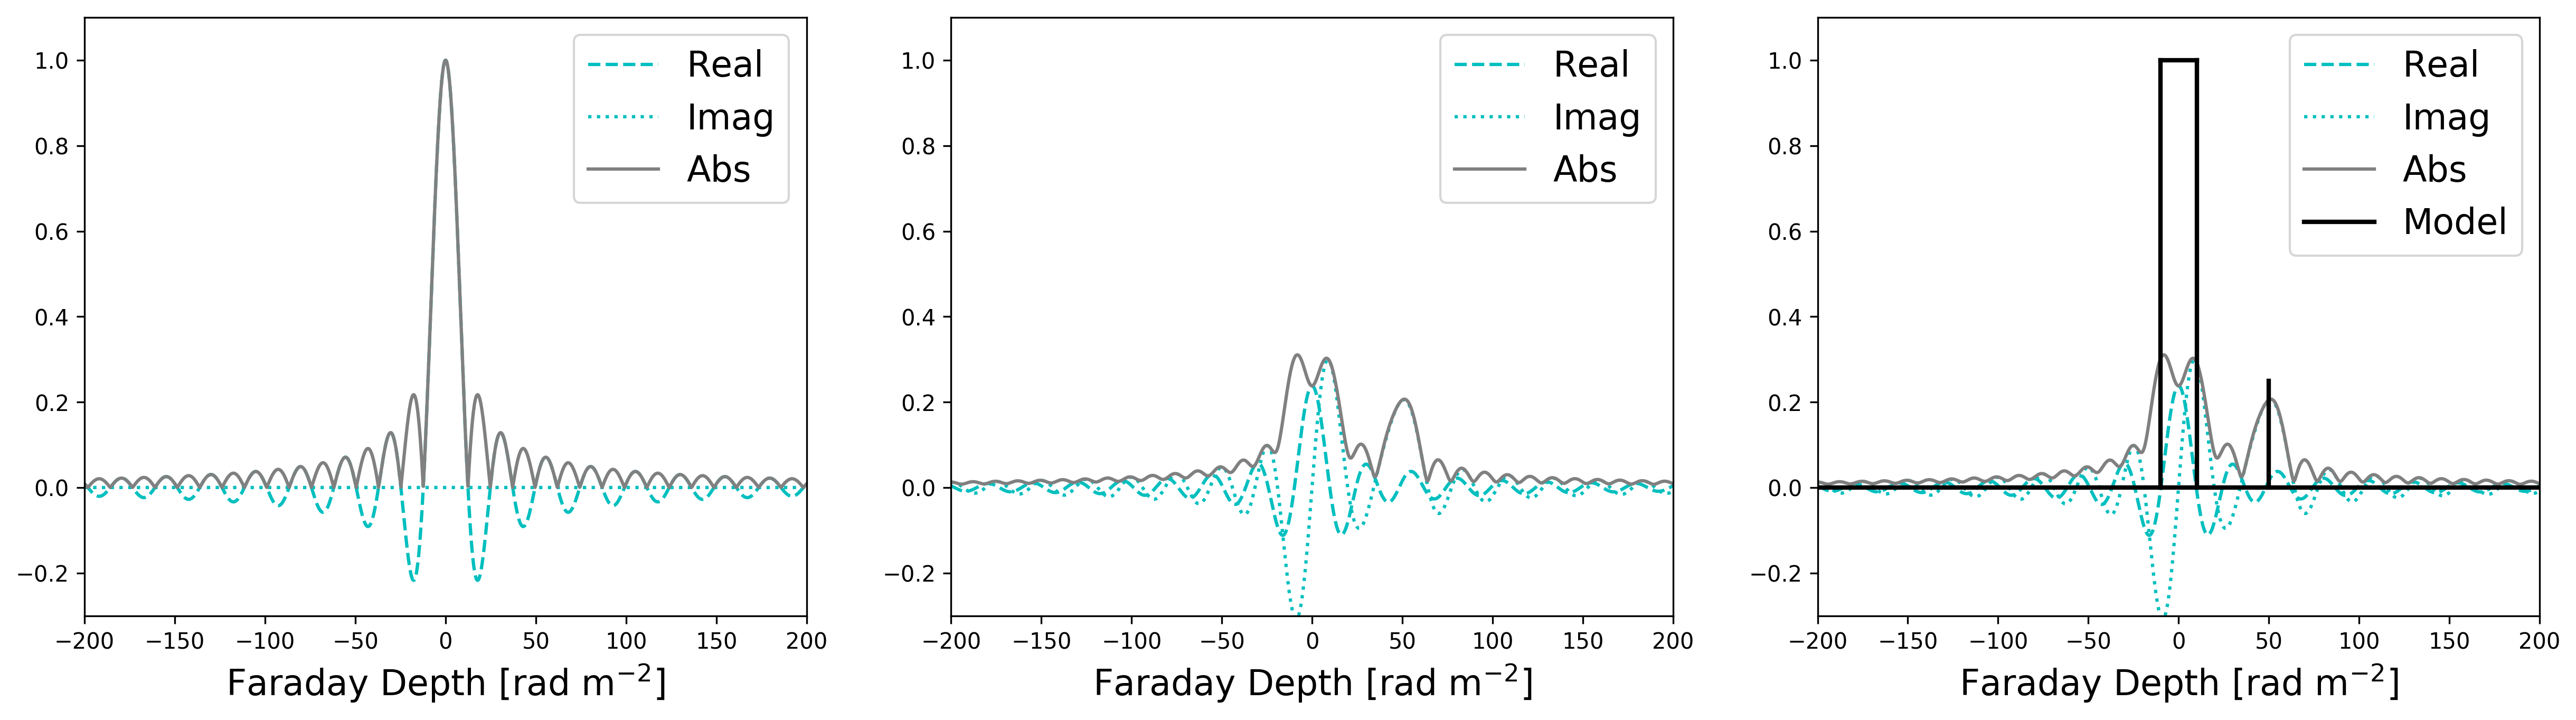
\includegraphics[width=0.9\textwidth]{./FIGURES/Scenario2_lsamp.png}}
\caption{\label{fig:scen2samp} Scenario 2: RMTF (left), Faraday depth spectrum (centre) and Faraday depth spectrum overlaid with input model (right) for the case of (i) data evenly sampled in frequency (top) and (ii) data evenly sampled in wavelength-squared (bottom). Data are noiseless in both cases.}
\end{figure*}

In what follows, we use inverse variance weights for calculating Faraday depth spectra. For the optimised GP reconstructions, the predictive variance used for the weights is given by
%
\begin{equation}
\label{eq:gpvar}
\sigma_{\ast}^2 = C_{\ast} + \sigma_{\rm n}^2,
\end{equation}
%
\citep{3569} where $\sigma_{\rm n}^2$ is the amplitude of the white noise kernel in Equation~\ref{eq:whitekernel}. The white noise variance needs to be included because we are building a Faraday depth spectrum from the prediction of the {\it noisy} complex polarization data.

\subsection{Parameter Estimation}
\label{sec:optimization}

To optimize the hyper-parameters of our GP kernel we use MCMC implemented via the {\sc emcee} package \citep{emcee} to explore the posterior probability distribution. We use 500 samples for a burn-in then take the maximum likelihood hyper-parameter values from the burn-in and perturb them by adding noise at a level of $10^{-5}$. We then use these perturbed values to start a production run of 5000 samples. Prior ranges for each of the hyper-parameters are shown in Table~\ref{tab:priors}. The lower limit on $\log P$ corresponds to a maximum Faraday depth of $\sim1200$\,rad\,m$^{-2}$.
%
\begin{table}
\caption{\label{tab:priors} Range of uniform priors used for each of the hyper-parameters in GP kernel, see Equation~\ref{eq:celkernel}.}
\centering
\begin{tabular}{|c|c|}
\hline
Hyper-parameter & Prior \\\hline
$\ln h$ & (-25,5)\\
$\ln c$ & (-25,5)\\
$\ln P$ & (-6,10)\\
$\ln \sigma$ & (-25,5)\\\hline
\end{tabular}
\end{table}


\subsection{Imputation of Missing Data}
\label{sec:missing}

The main objective of replacing missing data points with their optimized mean values from the GP model is to improve the interpretability of the resulting Faraday depth spectra. RFI flagging creates gaps in the polarization data thereby reducing the $\lambda^{2}$-coverage in an irregular fashion and causing the sidelobe structure in the RMTF to become more prominent.
%
\begin{figure*}
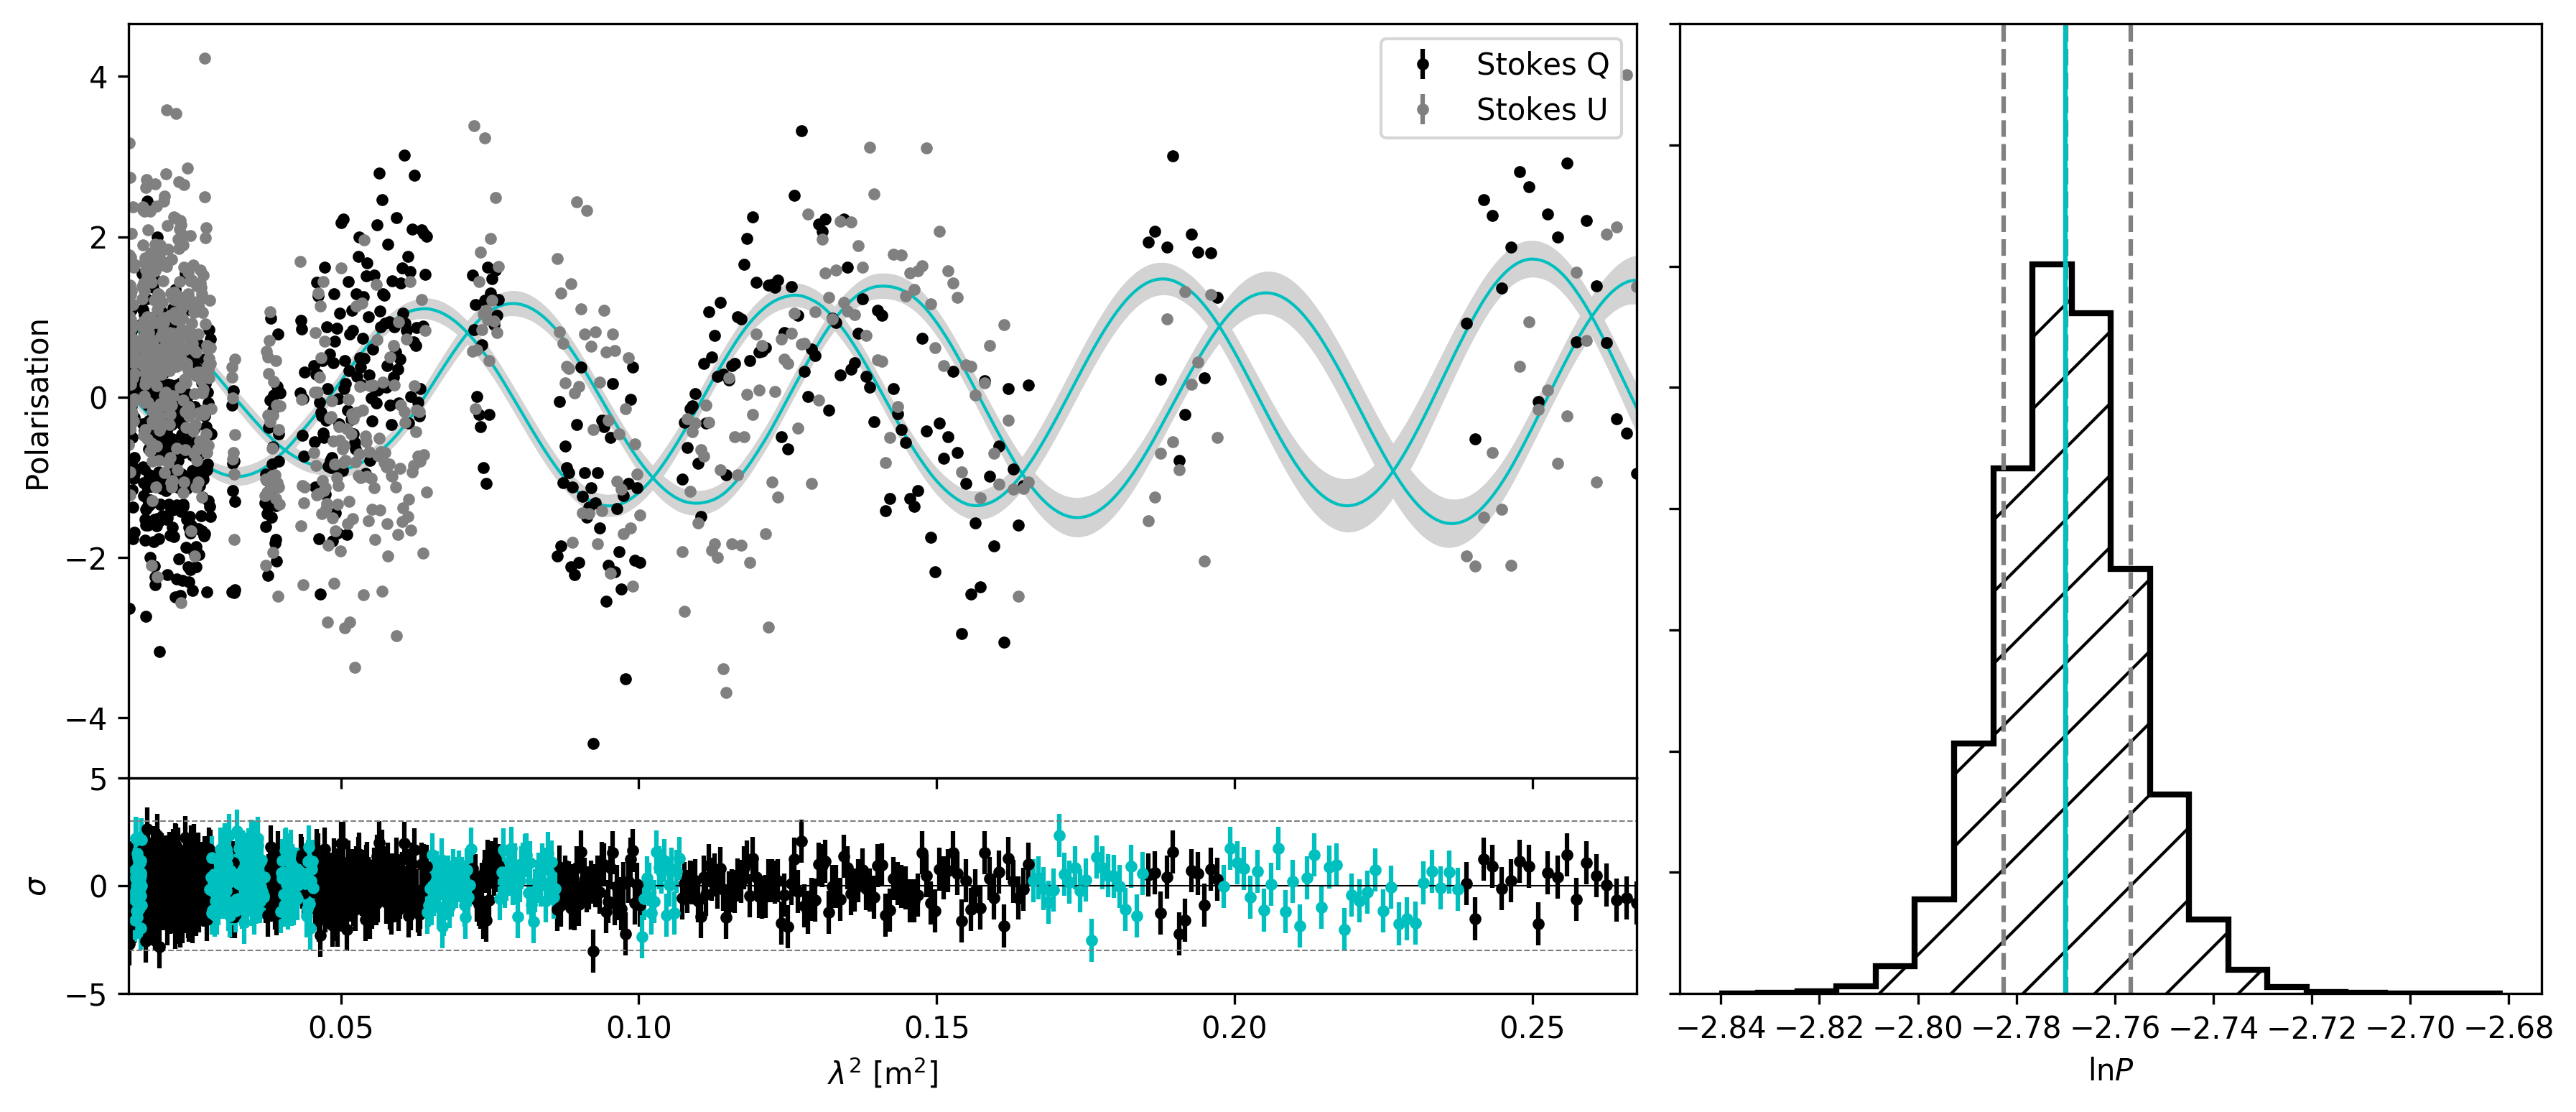
\includegraphics[width=0.9\textwidth]{./FIGURES/diff_case1_minus40_n1.png}
\caption{\label{fig:scenario1} Left upper: Stokes parameters for Scenario 1 (see \S~\ref{sec:scenarios}) with SNR$_{\rm chan}=1$ and 40\% of the data flagged; black \& grey error bars), and maximum a posteriori GP model (Equation~\ref{eq:celkernel}; blue solid line) with one standard deviation posterior uncertainty (grey shaded area). Left lower: residuals between the posterior mean for Stokes Q and the data (black points) and residuals between the posterior mean and the missing/flagged Stokes Q data (blue points). The $\pm3\sigma$ limits are marked by grey dashed lines. Right: The inferred period of the process with the true period marked (vertical blue line) as well as the 16\%, 50\% and 84\% confidence intervals of the posterior probability distribution (grey dashed lines).}
\end{figure*}

To mimic the RFI flagging process, we remove random portions of data from the simulated data set. To do this, a random position in the data set is selected and a chunk comprised of a randomly selected number of entries is removed. This process is repeated until the desired percentage of data is removed. We simulate data sets with 20\%, 30\% and 40\% missing values. An example of this flagging using the Scenario~1 dataset is shown in Figure~\ref{fig:scenario1}, which shows the input data, flagged at a level of 40\%. These data are scattered by white noise, giving a signal-to-noise of one in each channel. Figure~\ref{fig:scenario1} also shows the posterior mean prediction from GP model, optimized using only the unflagged data points, as well as the residual between the input data and the optimised GP model for both the unflagged and flagged data points. The right-hand panel of Figure~\ref{fig:scenario1} shows the posterior probability distribution for the hyper-parameter, $P$, which is used to calculate the rotation measure.

The effect of the flagging process on the Faraday depth spectrum is shown for Scenario~1 in Figure~~\ref{fig:flagging1}. In Figure~\ref{fig:flagging1}~(right), data have been imputed at regular intervals across the full bandwidth of the simulation and the Faraday depth spectrum calculated using the posterior mean values, weighted by the posterior covariance at each point. The Faraday depth spectra from the data shown in Figure~\ref{fig:scenario1} are displayed in Figure~\ref{fig:flagging1}~(bottom).
%
\begin{figure*}
\centerline{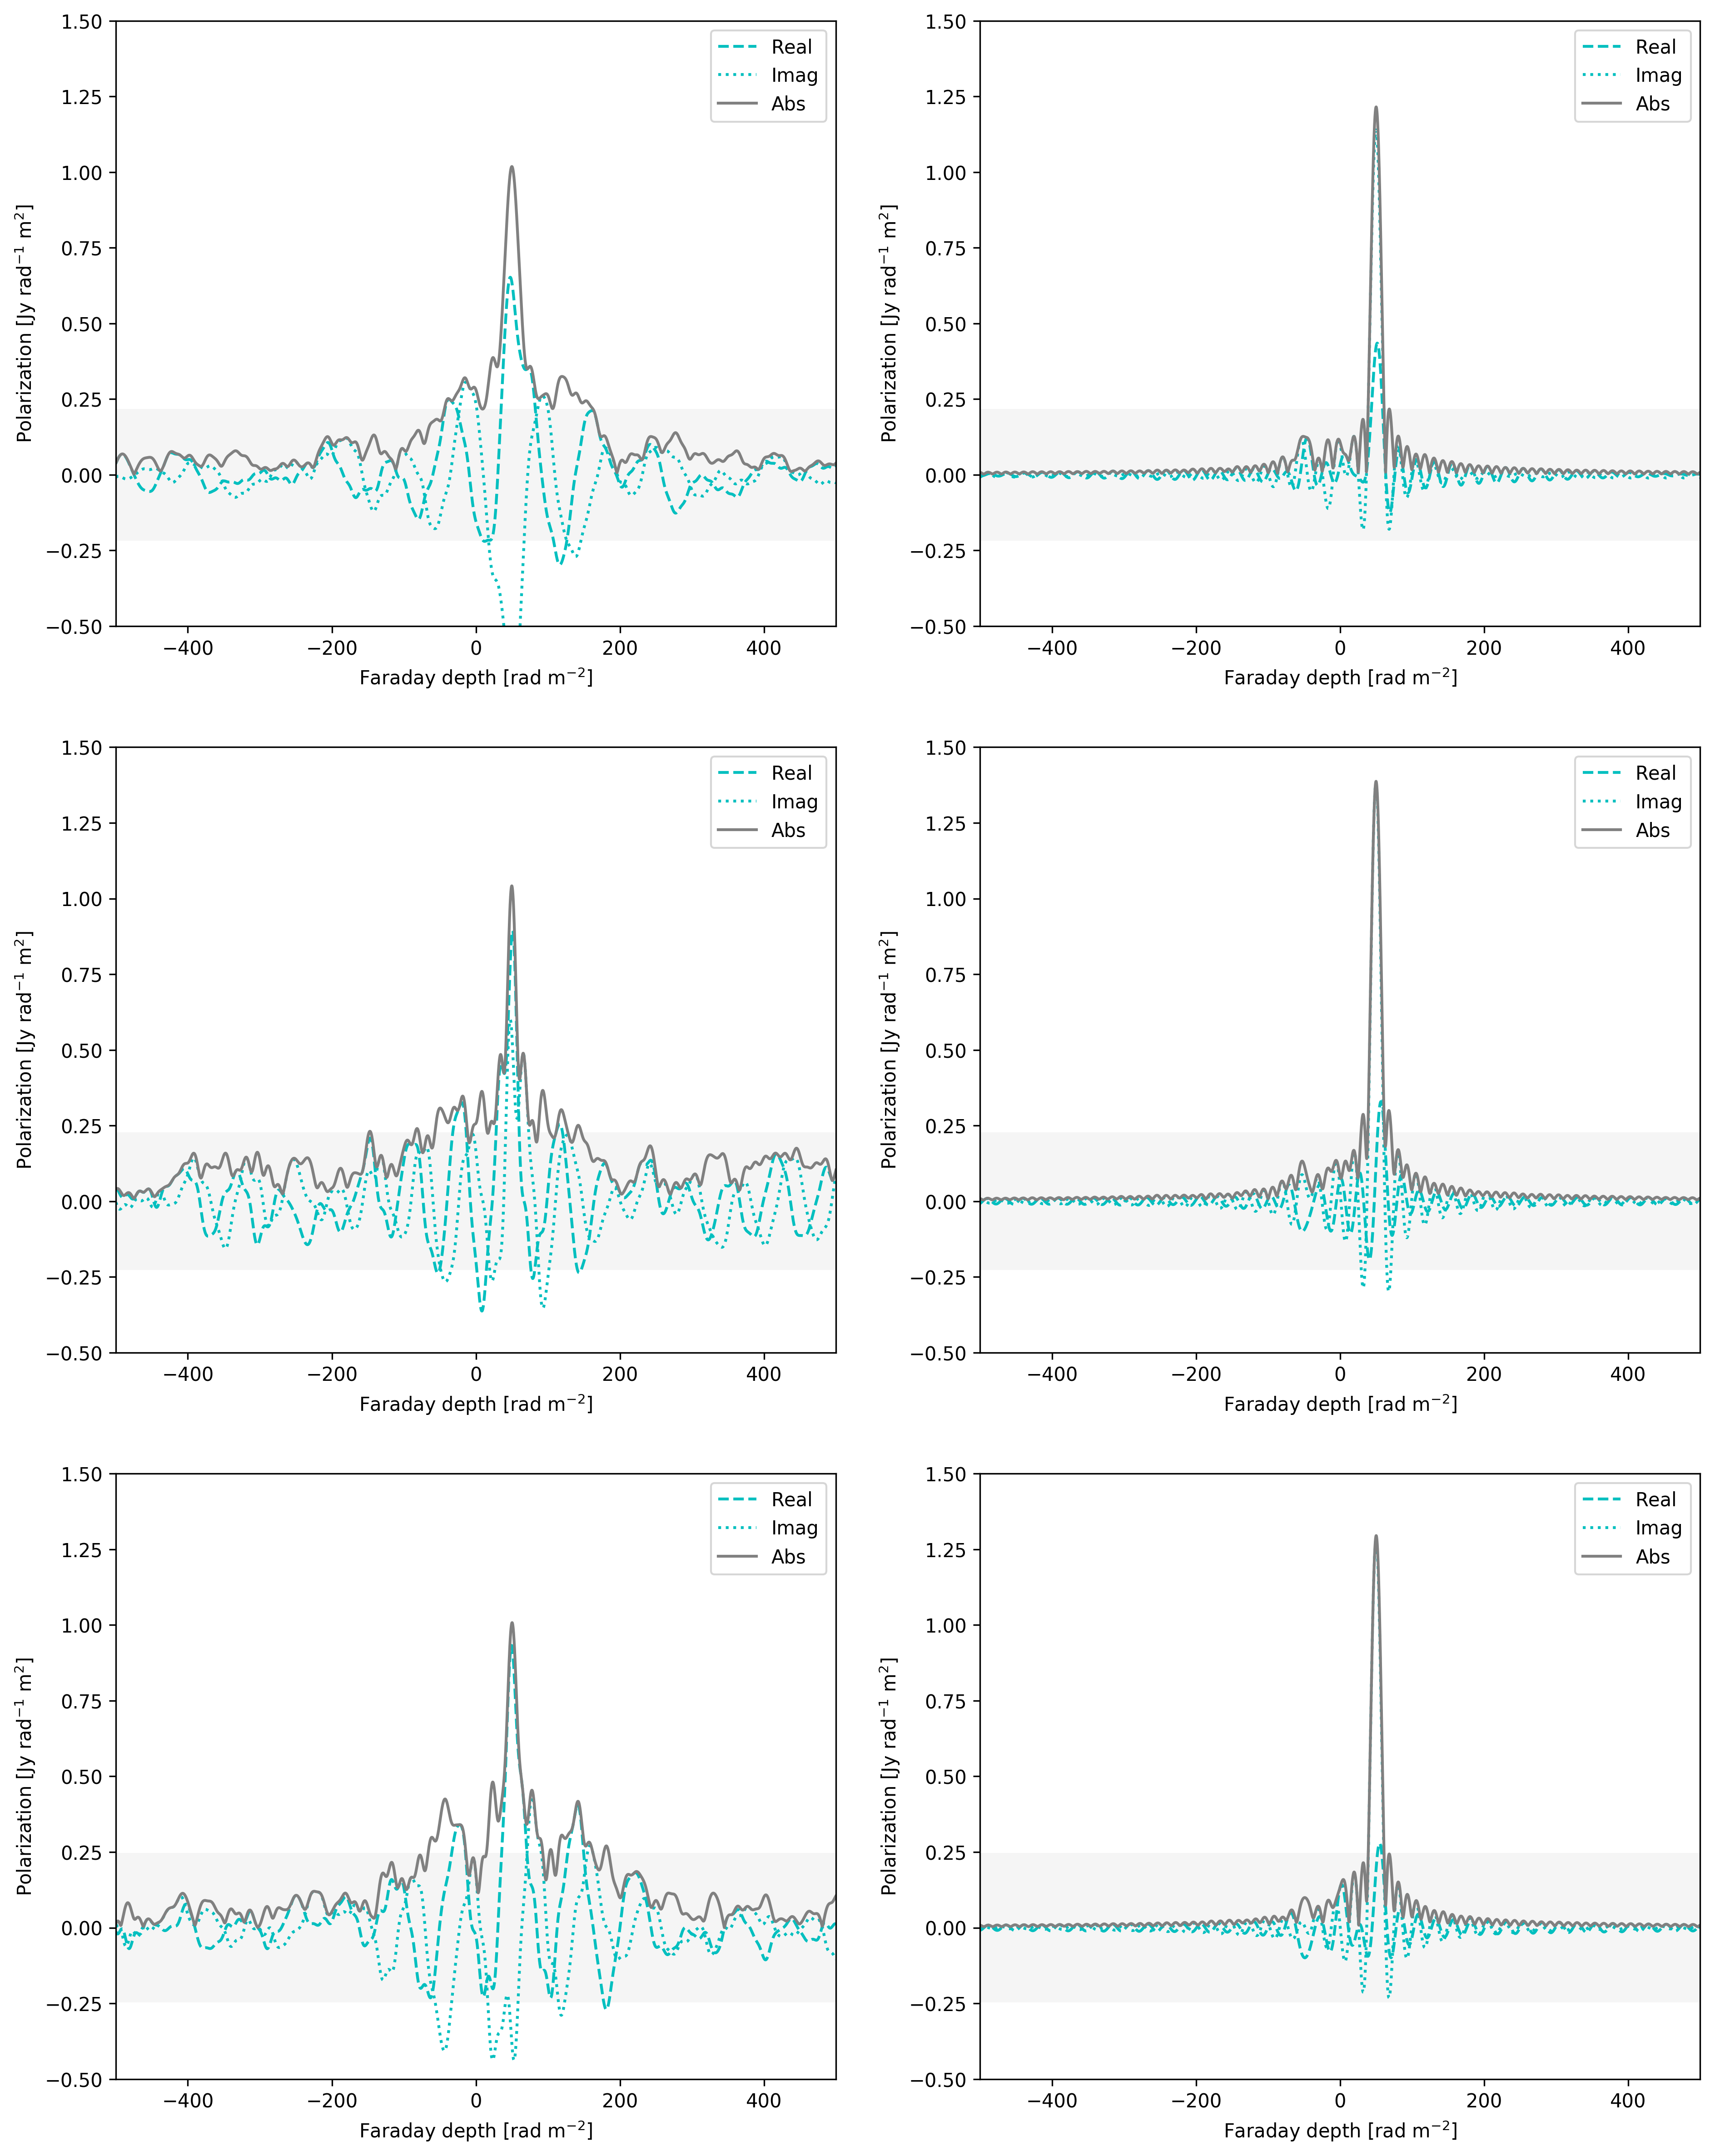
\includegraphics[width=0.95\textwidth]{./FIGURES/figure6.png}}
\caption{\label{fig:flagging1} Faraday depth spectra for Scenario~1 (Faraday thin) with 20\% (top), 30\% (middle) and 40\% (bottom) of channel data flagged and ${\rm SNR}_{\rm chan} = 1$. Left: Faraday depth spectrum from flagged data. Right: Faraday depth spectra from GPM reconstructed data as described in \S~\ref{sec:missing}. The $\pm$5\,$\sigma_{\phi}$ limits are shown as a light grey shaded area.}
\end{figure*}


It is noticeable in Figure~\ref{fig:flagging1} that the spectra calculated from the optimized GP model appear significantly cleaner than those calculated from the original data. This is in part because the sidelobe structure due to the gaps in frequency coverage is reduced, but also because the posterior mean values from the model are not scattered by the thermal noise in the same way as the original data. Although this may be advantageous in enhancing some features of the spectra, it can also potentially lead to over-interpretation of low-level features. We caution that structures present at amplitudes below $5-8\,\sigma_{\phi}$ should not be considered to represent true astrophysical components but are more likely to arise from structure in the noise. The value of $\sigma_{\phi}$ itself can be calculated from the white noise component of the GP model, or alternatively from the uncorrelated thermal measurement noise on Stokes~Q and Stokes~U if this is known a priori. In the case of Figure~\ref{fig:flagging1}, the $5\sigma_{\phi}$ bound is approximately $\pm0.2$\,Jy\,m$^2$\,rad$^{-1}$.


As illustrated by \cite{celerite}, it is often the case that valid inferences can be made using incorrect GP models. For physical processes whose underlying properties are not well understood, such as generalised Faraday spectra, this can significantly complicate the process of selecting a parametric model. Incorporating domain knowledge helps to make the problem of model selection and interpretation of parameters less difficult. We demonstrate this by using the GP model from Scenario~1 to impute missing data for simulations of Scenario~2. An example of this is shown in Figure~\ref{fig:scenario2}, which shows a simulated dataset where 20\% of the data points have been removed to mimic RFI flagging. In spite of not being an exact model, the optimized GP is able to reconstruct the missing data within the measurement uncertainties. It can also be seen that the optimized model is able to recover the rotation measure of the radio galaxy with high accuracy.
%
\begin{figure*}
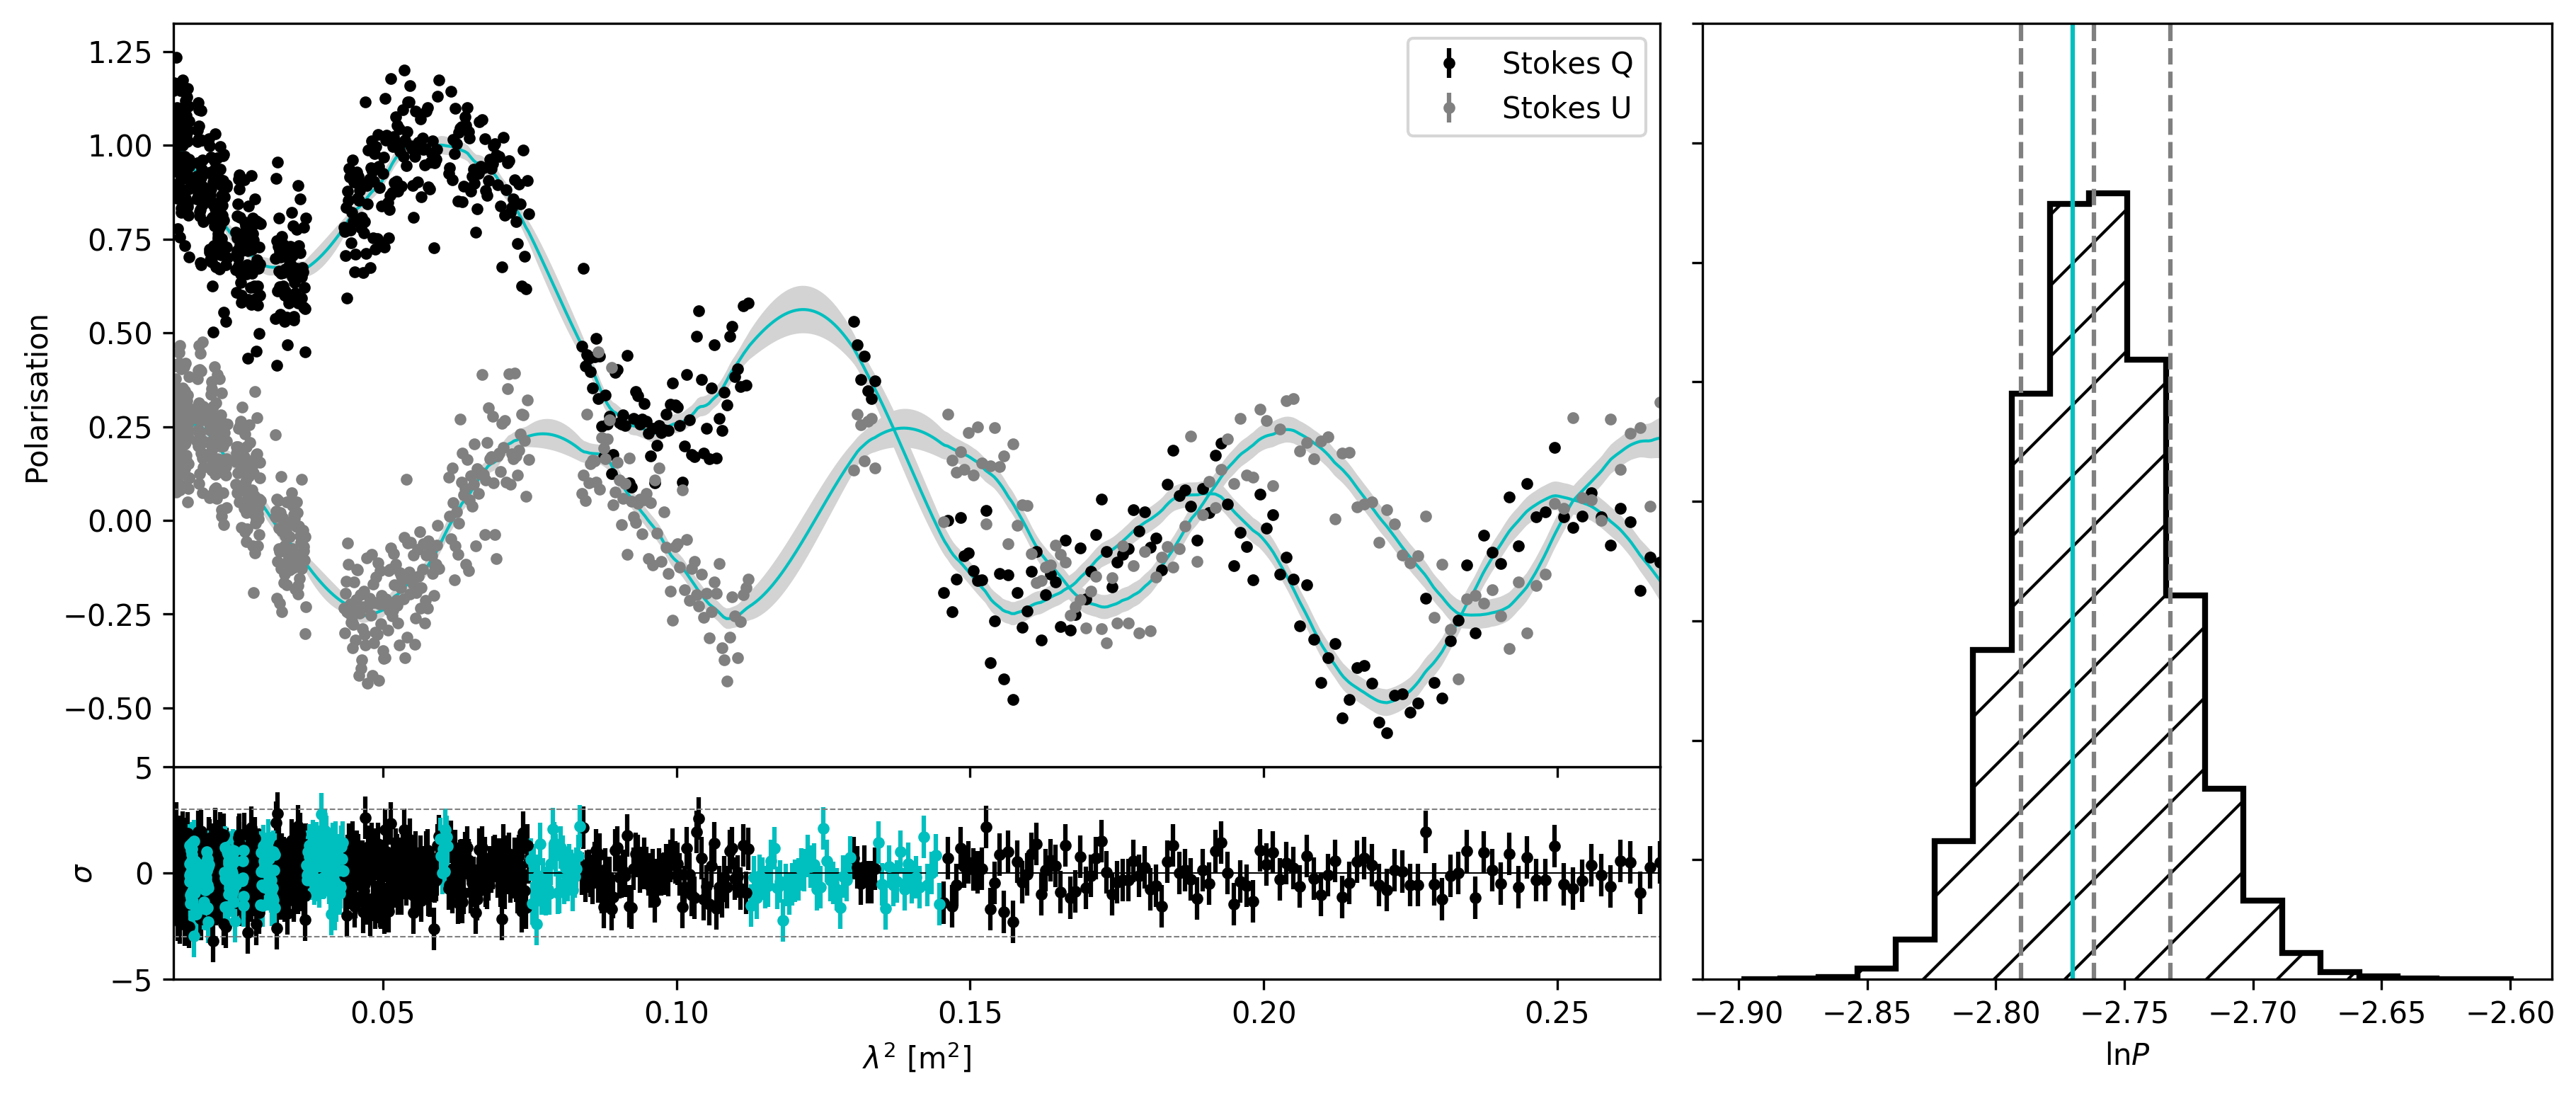
\includegraphics[width=0.9\textwidth]{./FIGURES/diff_case2_minus30_n0p1.png}
\caption{\label{fig:scenario2} Left upper: Stokes parameters for Scenario 2 (see \S~\ref{sec:scenarios}); black \& grey error bars), and maximum a posteriori GP model (Equation~\ref{eq:celkernel}; blue solid line) with one standard deviation posterior uncertainty (grey shaded area). Left lower: residuals between the posterior mean for Stokes Q and the data (black points) and residuals between the posterior mean and the missing/flagged Stokes Q data (blue points). The $\pm3\sigma$ limits are marked by grey dashed lines. Right: The inferred period of the process with the true period marked (vertical blue line) as well as the 16\%, 50\% and 84\% confidence intervals of the posterior probability distribution (grey dashed lines).}
\end{figure*}

In this case, recovering the Faraday depth of the thin component is not as strong an indicator of performance as in Scenario~1. Instead we compare the posterior prediction of the optimized GP to the input model without noise. The input model is shown in Figure~\ref{fig:scenario2} as a black dashed line. Figure~\ref{fig:flagging2} shows the Faraday depth spectrum reconstructed from the optimized GP for Scenario~2 in the presence of different levels of RFI flagging. These should be compared to the noiseless model spectrum shown in Figure~\ref{fig:scen2samp}.
%
\begin{figure*}
%\centerline{Original data \hskip 0.45\textwidth Imputed data}
\centerline{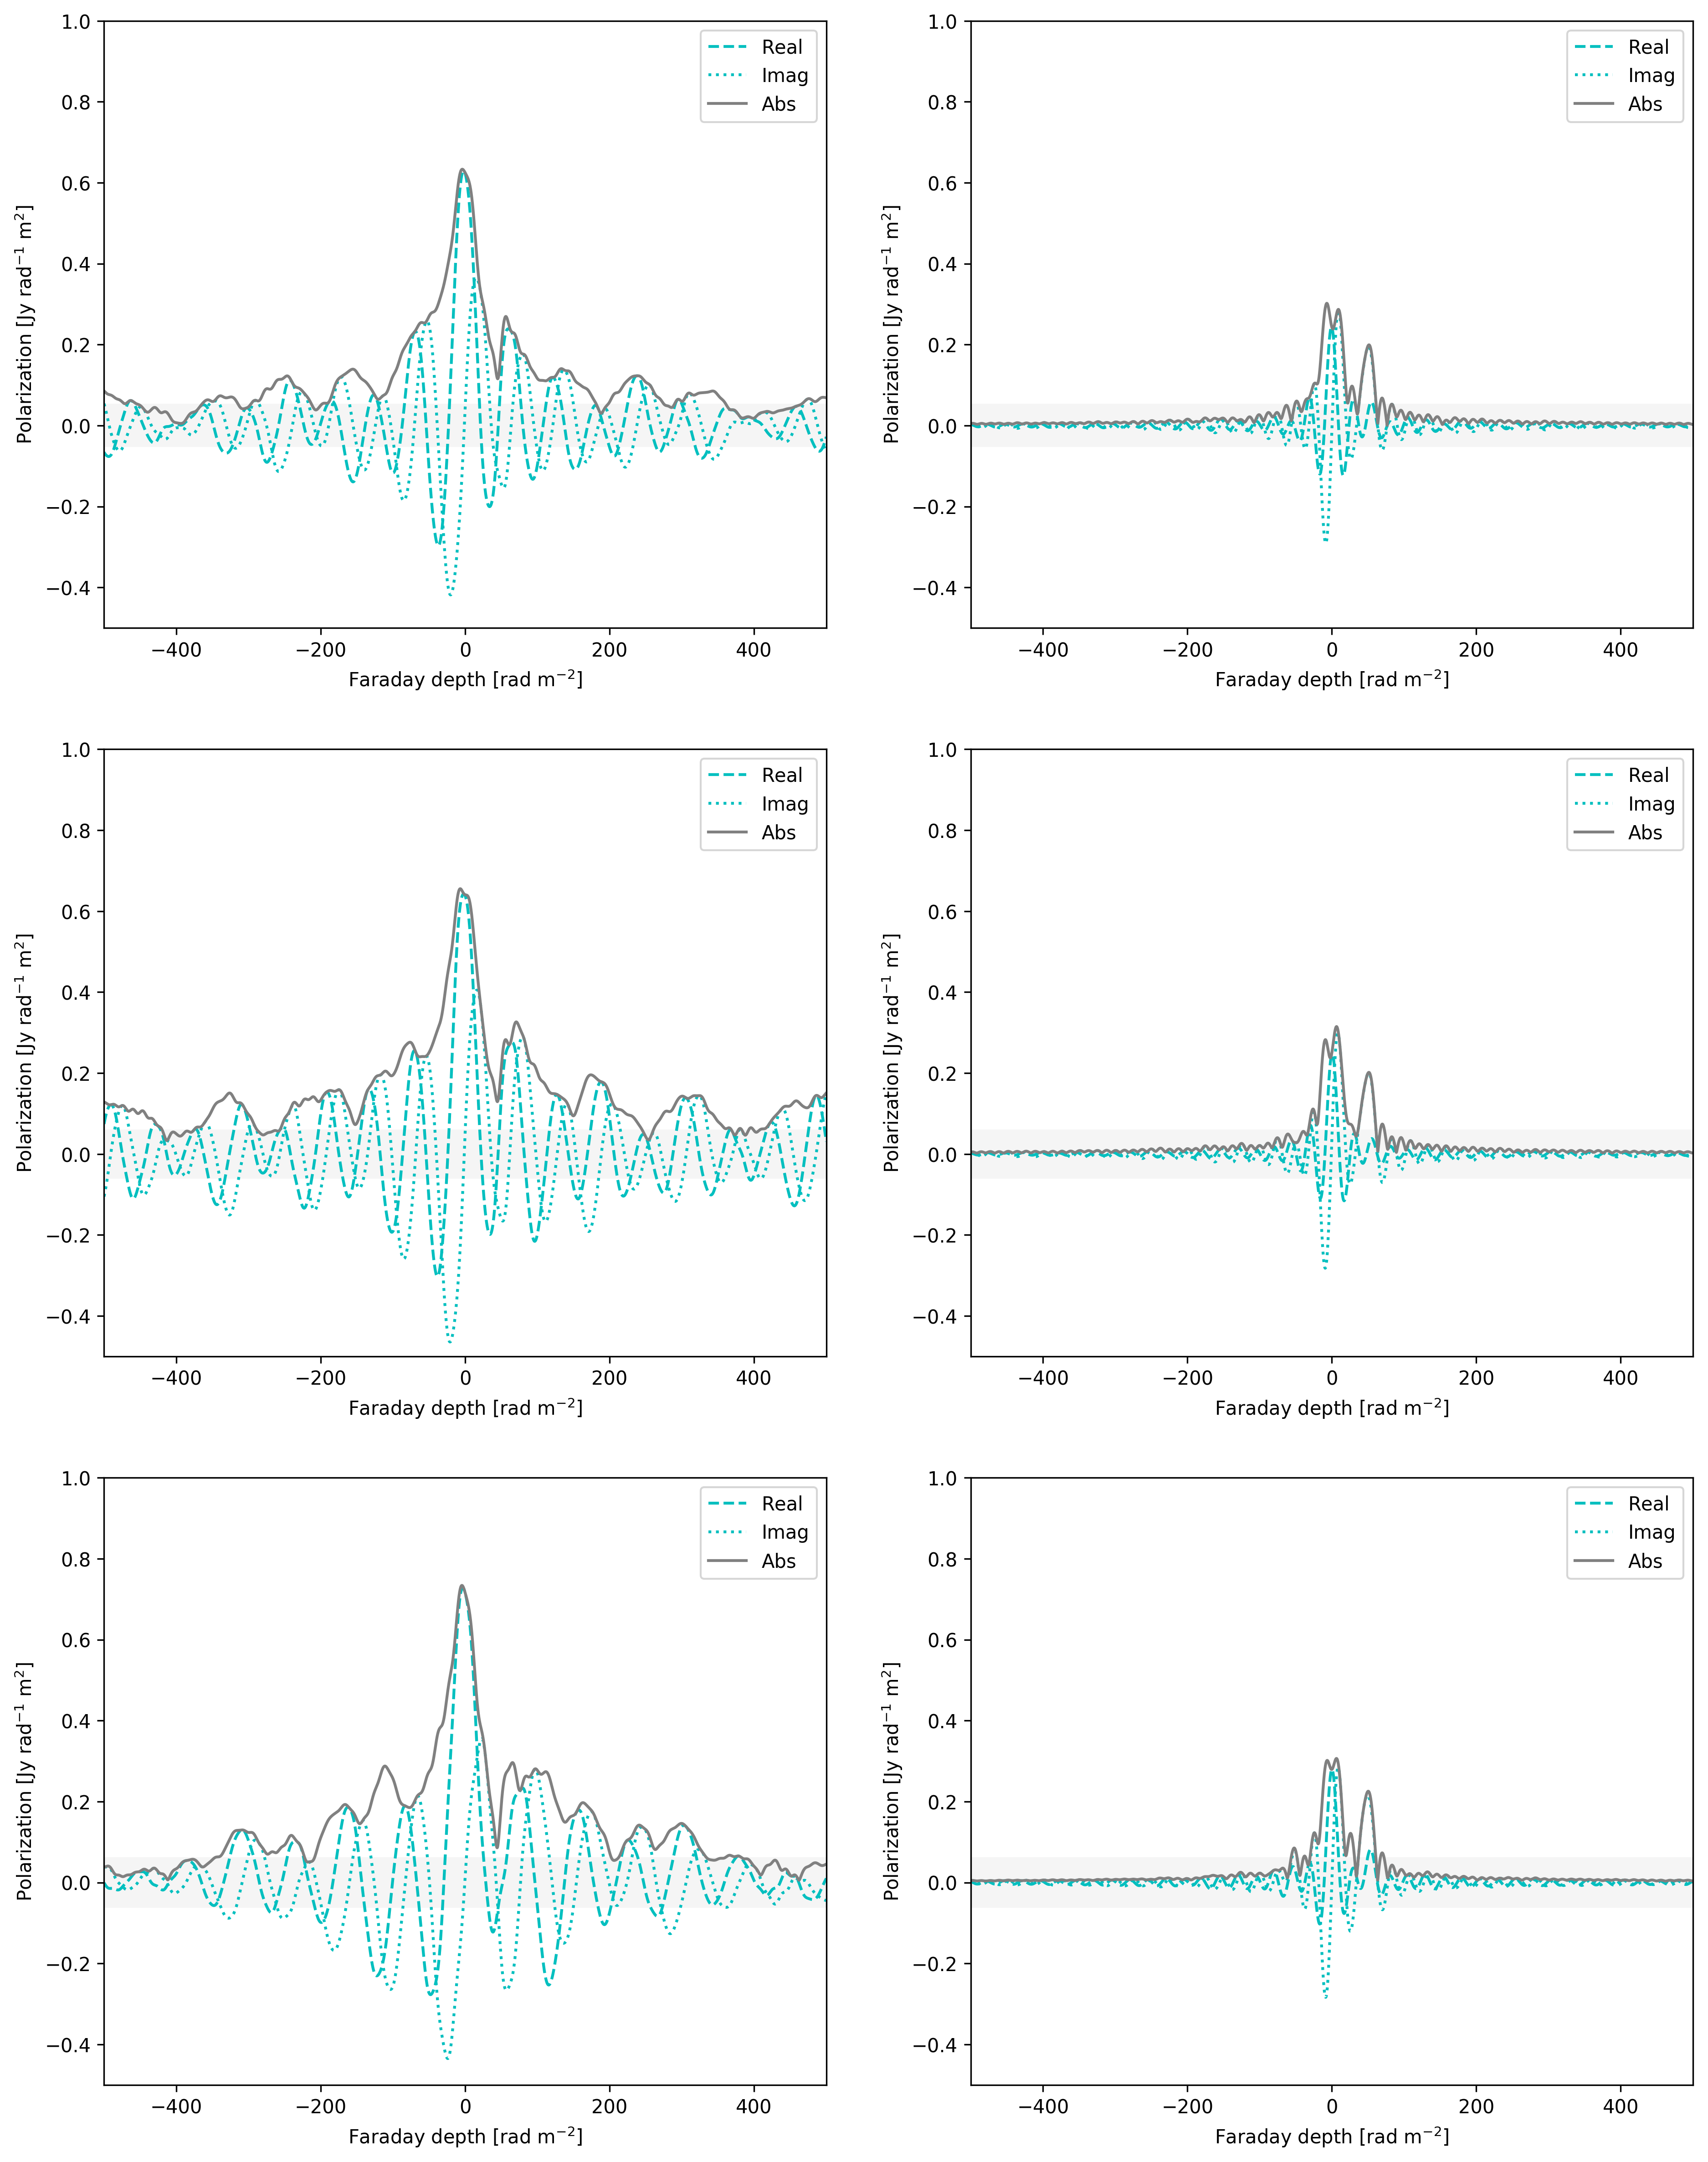
\includegraphics[width=0.95\textwidth]{./FIGURES/figure8.png}}
\caption{\label{fig:flagging2} Faraday depth spectra for Scenario~2 (Faraday complex) with 20\% (top), 30\% (middle) and 40\% (bottom) of channel data flagged and ${\rm SNR}_{\rm chan, U} = 1$. Left: Faraday depth spectrum from flagged data. Right: Faraday depth spectra from GPM reconstructed data as described in \S~\ref{sec:missing}. The $\pm$5\,$\sigma_{\phi}$ limits are shown as a light grey shaded area.}
\end{figure*}

%\subsection{Recovery of Faraday Thick Structure}
%\label{sec:thick}

%As shown in Equation~\ref{eq:fdscale}, the sensitivity of a measured Faraday depth spectrum, $F(\phi)$, to extended or thick structures of a particular scale along the line of sight is governed by the minimum value of wavelength-squared sampled by the measurement. This inverse relationship means that data which are are observed at shorter wavelengths will have greater sensitivity to larger scale Faraday thick structures. However, due to the limitations on recoverable fractional bandwidth in radio astronomy receiver systems, these observations will also generally suffer from poorer resolution in Faraday depth.

%Gaussian processes have historically been used for forward prediction of time series in a number of different applications [REFs]. Here we demonstrate that by making a prediction of the posterior mean at wavelengths smaller than the minimum observable wavelength GPs can be used to improve the recovery of extended structures in Faraday depth space.  This is illustrated in Figure~\ref{fig:extended} (top), where Stokes~Q and Stokes~U data have been predicted at values of $\lambda^2$ up to two orders of magnitude smaller than the measured $\lambda^2_{\rm min}$. The resulting Faraday depth spectrum is shown in Figure~\ref{fig:extended} (bottom), where the improvement in structure definition is clearly seen for the GP reconstructed spectrum relative to the Faraday depth spectrum calculated from the original measurements. The more detailed discussion of these results is presented in \S~\ref{sec:disc}.
%
%\begin{figure*}
%\centerline{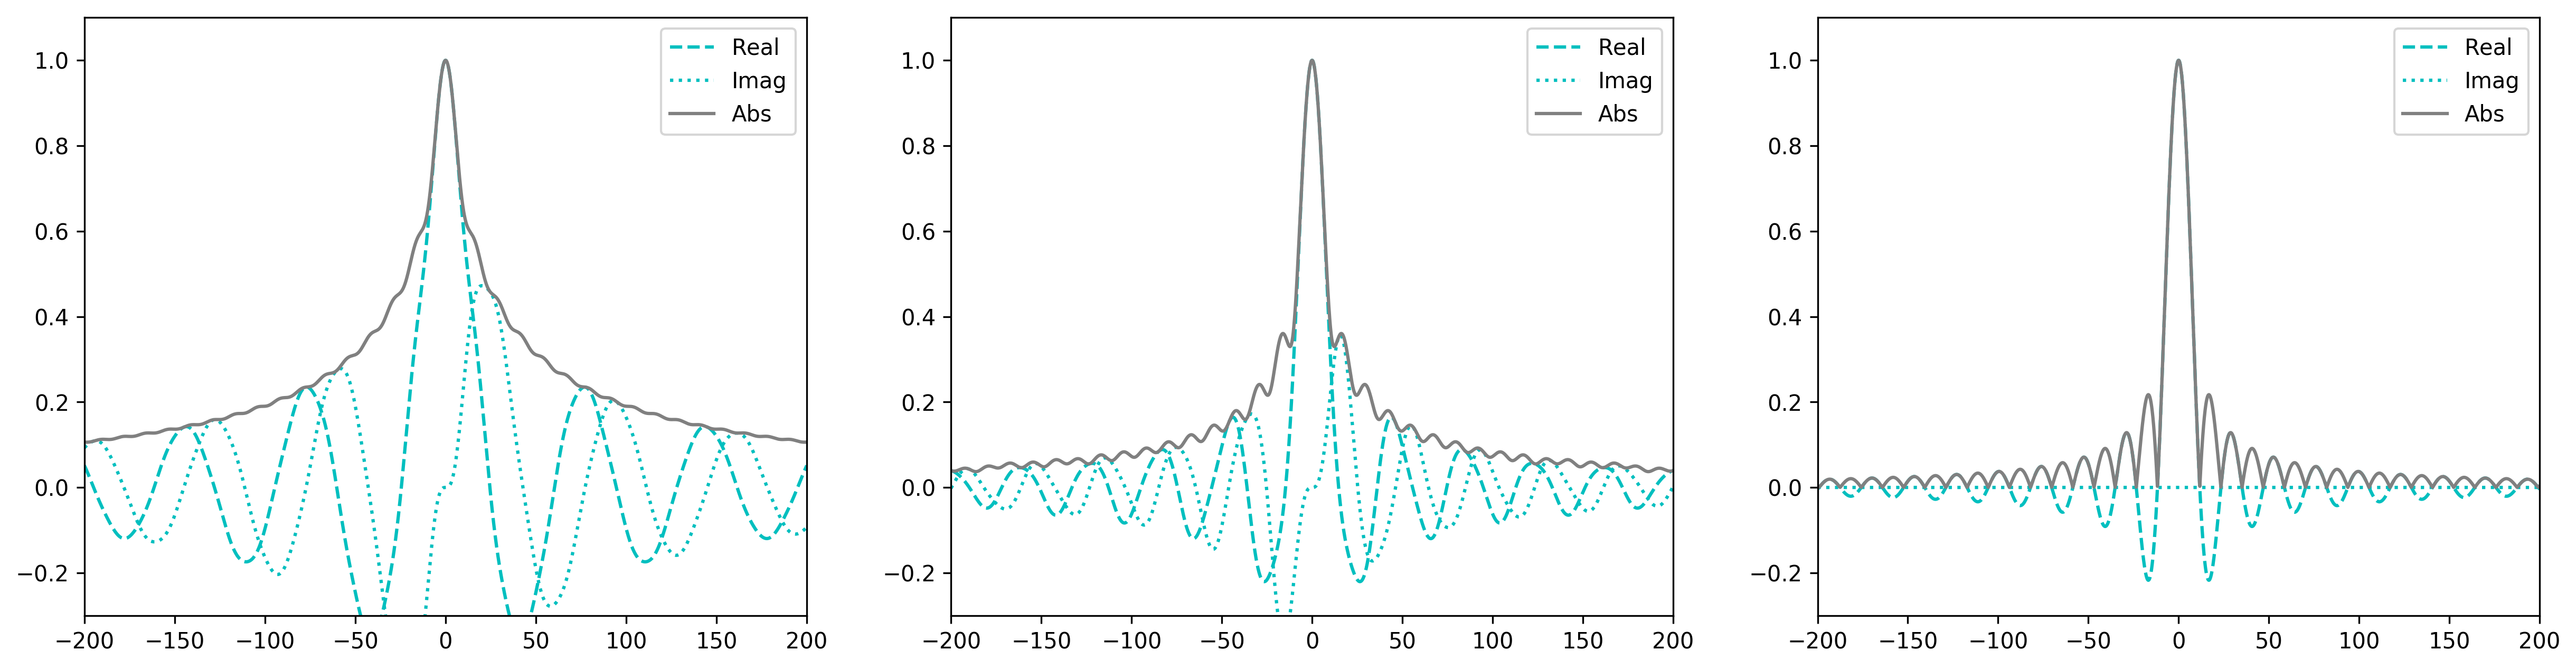
\includegraphics[width=0.9\textwidth]{./FIGURES/3rmtf_l0.png}}
%\centerline{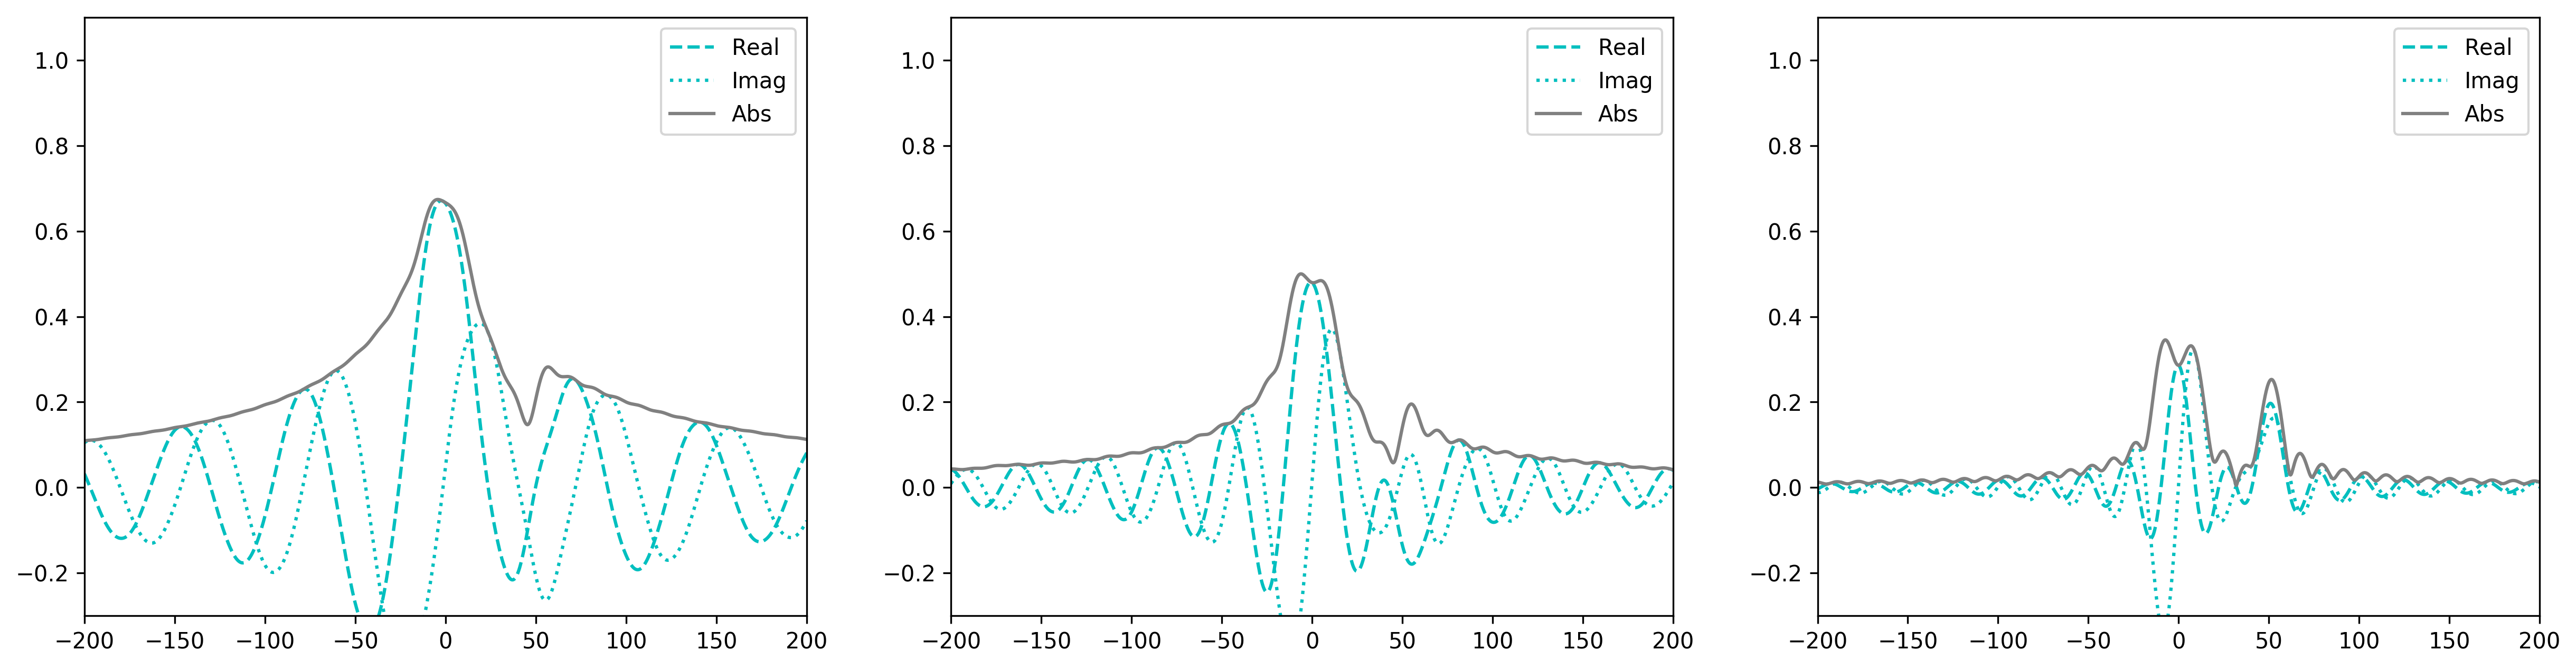
\includegraphics[width=0.9\textwidth]{./FIGURES/3fspec_l0.png}}
%\caption{\label{fig:scen2extend} Scenario 2: RMTF (top left) and Faraday depth spectrum (bottom left) for data uniformly sampled in frequency; RMTF (top centre) and Faraday depth spectrum (bottom centre) for data uniformly sampled in $\lambda^2$ in the range $0\le \lambda^2 \le \lambda^2_{\rm max}$ with weights from the posterior covariance; RMTF (top right) and Faraday depth spectrum (bottom right) for data uniformly sampled in $\lambda^2$ in the range $0\le \lambda^2 \le \lambda^2_{\rm max}$ with all weights set to unity. Data are noiseless in all cases.}
%\end{figure*}

\subsection{Multiple Sources along the line of sight}
\label{sec:multiple}

As described in \cite{Sun_2015}, it is expected that many lines of sight will have more than one Faraday thin component. Such Faraday geometries are also able to be recovered by the kernel in Equation~\ref{eq:celkernel}. In this case the hyper-parameter $P$ will represent the $|RM|$ of the component with the highest rotation. An example of where this can occur is the super-position of radio galaxy jets or lobes oriented along a line of sight unresolved by the beam of a telescope. Such geometries result in double Faraday components, typically with similar Faraday depths as the integrated rotation differs only by the degree contributed in the local medium between the jets whilst experiencing a common degree of rotation from the comparatively larger path between the galaxy and the observer. An example of such a situation is shown in Figure~\ref{fig:double}. We illustrate the GP model in this figure at high signal to noise, SNR$_{\rm chan} = 20$, to show that the GP can accurately represent the complex polarization behaviour of multiple sources without requiring additional kernel components. The Faraday depth spectra in Figure~\ref{fig:double} show the recovered Faraday depth spectrum from the noisy input data (left) and from the optimised GP reconstruction (right). It can be observed that the double structure is more apparent in the GP reconstruction. We note that the separation of the peaks in Faraday depth is wider than the separation of components in the model. This is not an artefact of the GP reconstruction, but due to the position of the first null in the RMTF.
%
\begin{figure*}
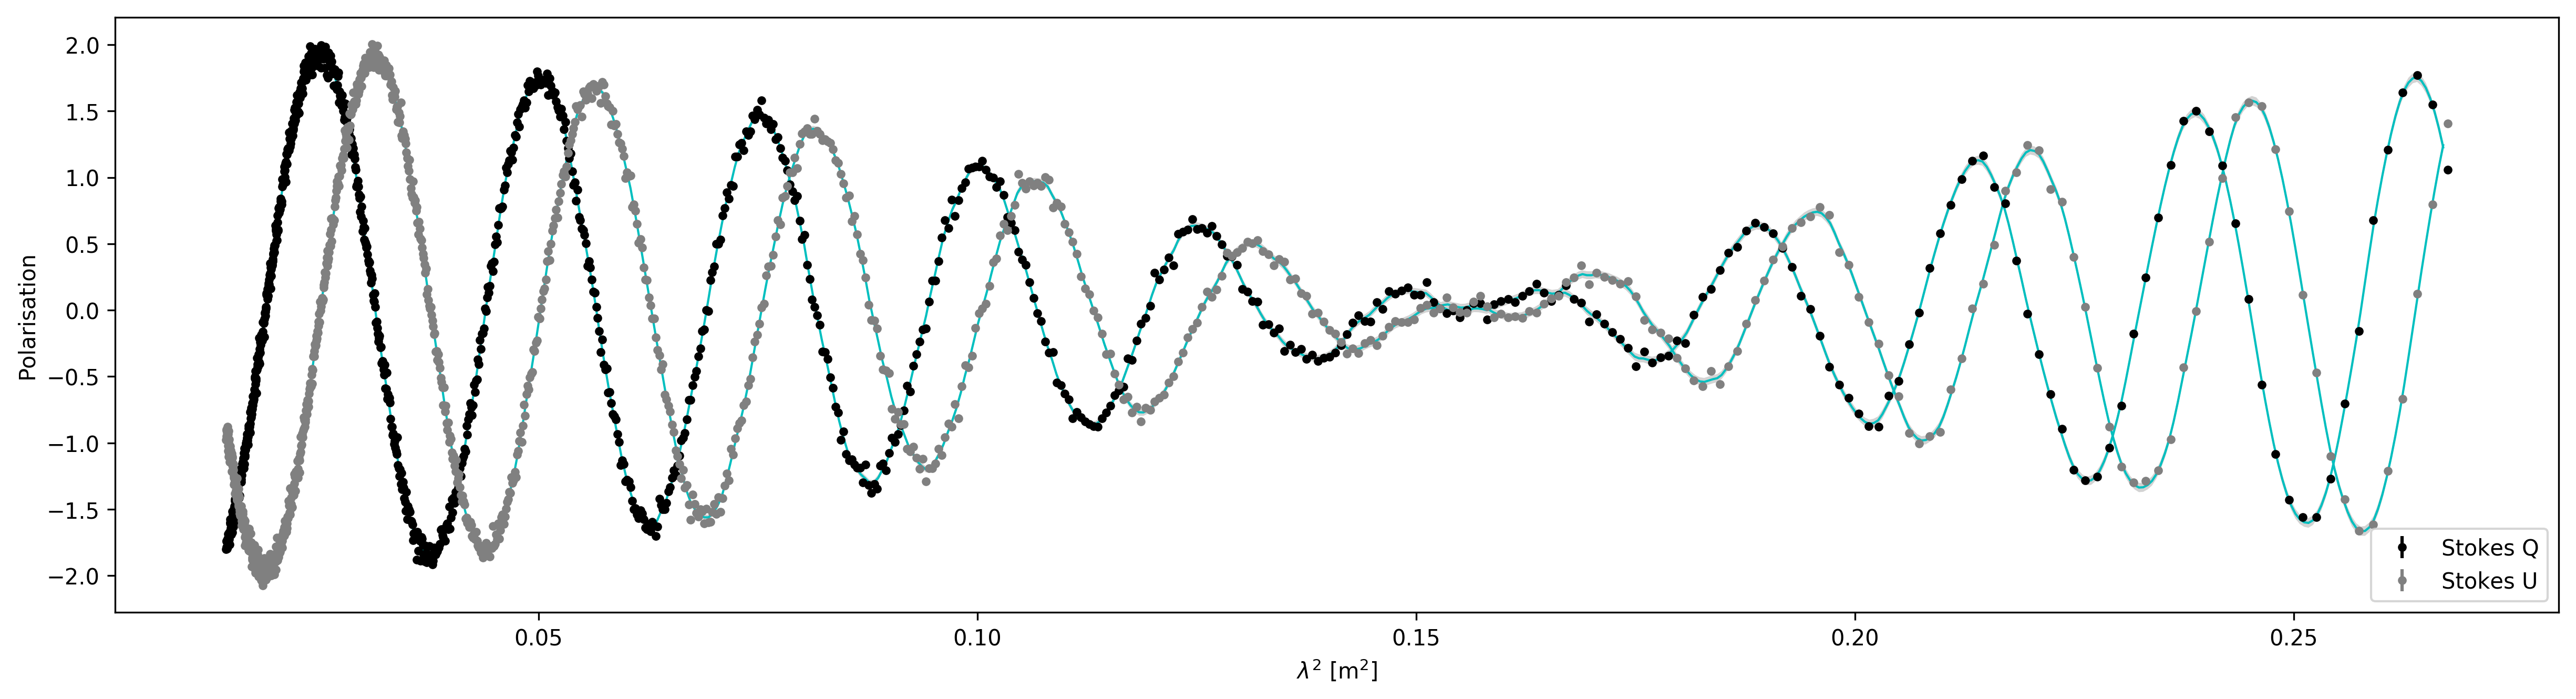
\includegraphics[width=0.88\textwidth]{./FIGURES/double_qu.png}
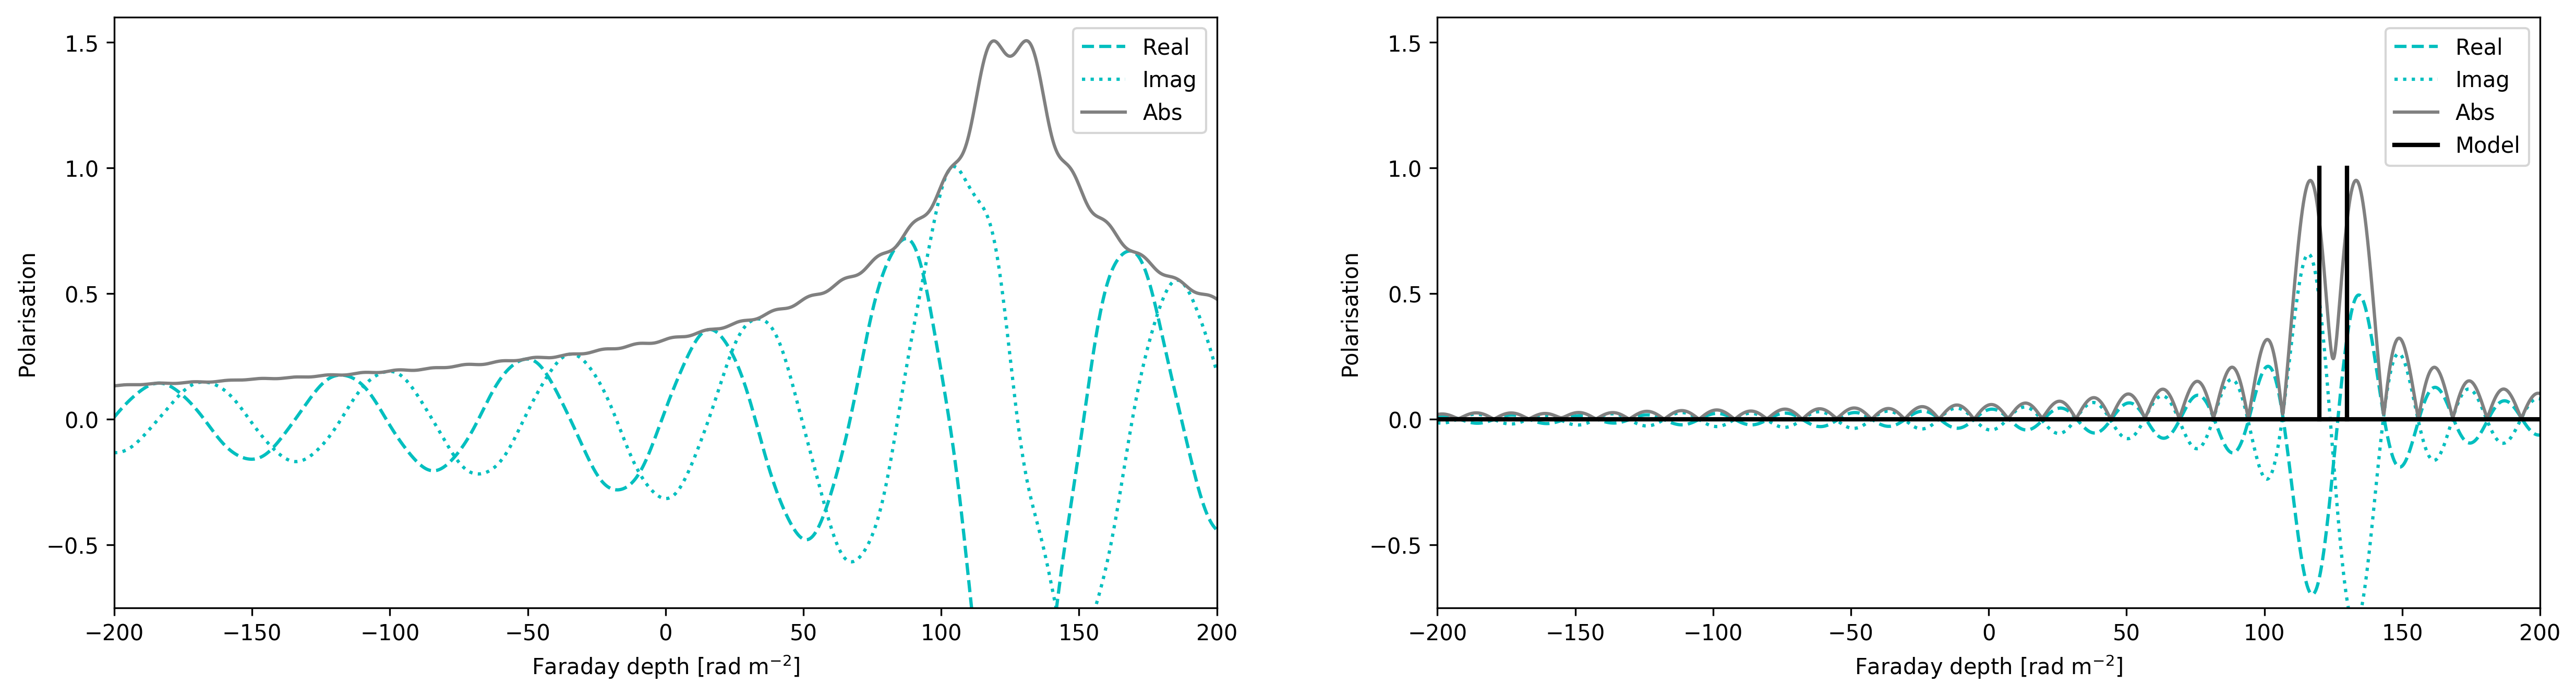
\includegraphics[width=0.9\textwidth]{./FIGURES/diff_double.png}
\caption{\label{fig:double} Upper: Stokes parameters for line of sight comprised of two Faraday thin sources with SNR$_{\rm chan}=20$ (black \& grey error bars), and maximum a posteriori GP model (Equation~\ref{eq:celkernel}; blue solid line) with one standard deviation posterior uncertainty (grey shaded area). Left lower: Faraday depth spectrum calculated from the noisy input data sampled at regular intervals in frequency. Right lower: Faraday depth spectrum calculated from the optimised GPM sampled at regular intervals in $\lambda^2$-space with the model components marked as solid black lines.}
\end{figure*}

 \subsection{Rotation Measure Extraction}
\label{sec:rms}

Under certain circumstances it is possible to use the optimised hyper-parameters to recover the rotation measure of a source. In principle, for Faraday thin sources the absolute value of the rotation measure can be recovered from the periodicity using,
%
\begin{equation}
|{\rm RM}| = \frac{\pi}{P}.
\end{equation}
%
Due to the stationary nature of the covariance kernels, it is not possible to recover the sign of the rotation measure from the hyper-parameters of the covariance matrix; however, it can be recovered by comparing the correlation co-efficient, $c_{\rm corr}$, between (e.g.) the Stokes Q data and the Stokes U data shifted by $\pm\pi/2$ radians, $U^{\pm}$:
%
\begin{equation}
\label{eq:corr}
c_{\rm corr}^{\pm} = \langle Q,U^{\pm} \rangle.
\end{equation}

Using Scenario One, we evaluate the accuracy of RM recovery for the Faraday thin source as a function of the signal-to-noise (SNR) of the integrated polarization data, ${\rm SNR}_{\rm int}$. Following \cite{2018arXiv180604326S}, we define this value as
%
\begin{equation}
{\rm SNR}_{\rm int} = \sqrt{N_{\rm chan}} \times \frac{P_0}{\sigma_{\nu}},
\end{equation}
%
where $\sigma_{\nu}$ is the standard deviation of the random Gaussian noise added to each frequency channel and $N_{\rm chan}$ is the number of frequency channels. $P_0$ is the polarized amplitude at the reference frequency, taken in this case to be 1.4\,GHz. Noise is added independently to both Stokes Q and Stokes U data.

It can be seen in Figure~\ref{fig:rm_snr} that for Scenario~1, the rotation measure is recovered with $< 1\,\sigma$ deviation from the true value for even low values of ${\rm SNR}_{\rm int}<10$ where the signal-to-noise on an individual frequency channel, ${\rm SNR}_{\rm chan}\ll 1$. A minimum value of ${\rm SNR}_{\rm int}=8$ is typically used to identify sources in total polarization images, see e.g. \cite{george_stil_keller_2012}, and this value is marked in Figure~\ref{fig:rm_snr}. It can be seen that the optimized RM value is in good agreement with both the expectation value and the true value of the RM above this limit.

However, we note that when using this method to obtain an RM there is a lower limit on the absolute value of the rotation measure that can be reliably recovered. This limit is dependent on the both the frequency coverage of the observational data and the signal to noise ratio. At very low values of Faraday depth the degree of rotation in the complex polarization signal becomes smaller and causes a degeneracy between hyper-parameter $c$ in Equation~\ref{eq:celkernel} and the periodicity, $P$. This is exacerbated for data at higher frequencies where the rotation is more poorly sampled. This lack of rotation also causes the method for assigning the direction of the rotation measure described in Equation~\ref{eq:corr} to be less effective, as there are not guaranteed to be $\pm\pi/2$ radians of rotation present in the observed data. As this lower limit, $\phi_{\rm lim}$, is a strong function of frequency coverage, it is possible to determine it a priori for a particular telescope such that
%
\begin{equation}
\label{eq:rmlim}
    \phi_{\rm lim} = \frac{\pi}{4\Delta \lambda^2},
\end{equation}
%
where $\Delta \lambda^2$ is the coverage of the observational data in $\lambda^2$-space and the given expression corresponds to that coverage being equivalent to $\pi/2$\,radians for $\phi_{\rm lim}$.  A illustrated in Figure~\ref{fig:survey}, RM values above this limit are recovered reliably for SNR$_{\rm int}\ge 8$.

We emphasise that this limit is only applicable to the calculation of the rotation measure from the hyper-parameters and does not affect the improvement in the Faraday depth spectrum from GPM re-sampling or imputation, as shown in Figures~\ref{fig:scen2samp}, where structure at low Faraday depths is recovered equivalently well.
%
\begin{figure*}
\centerline{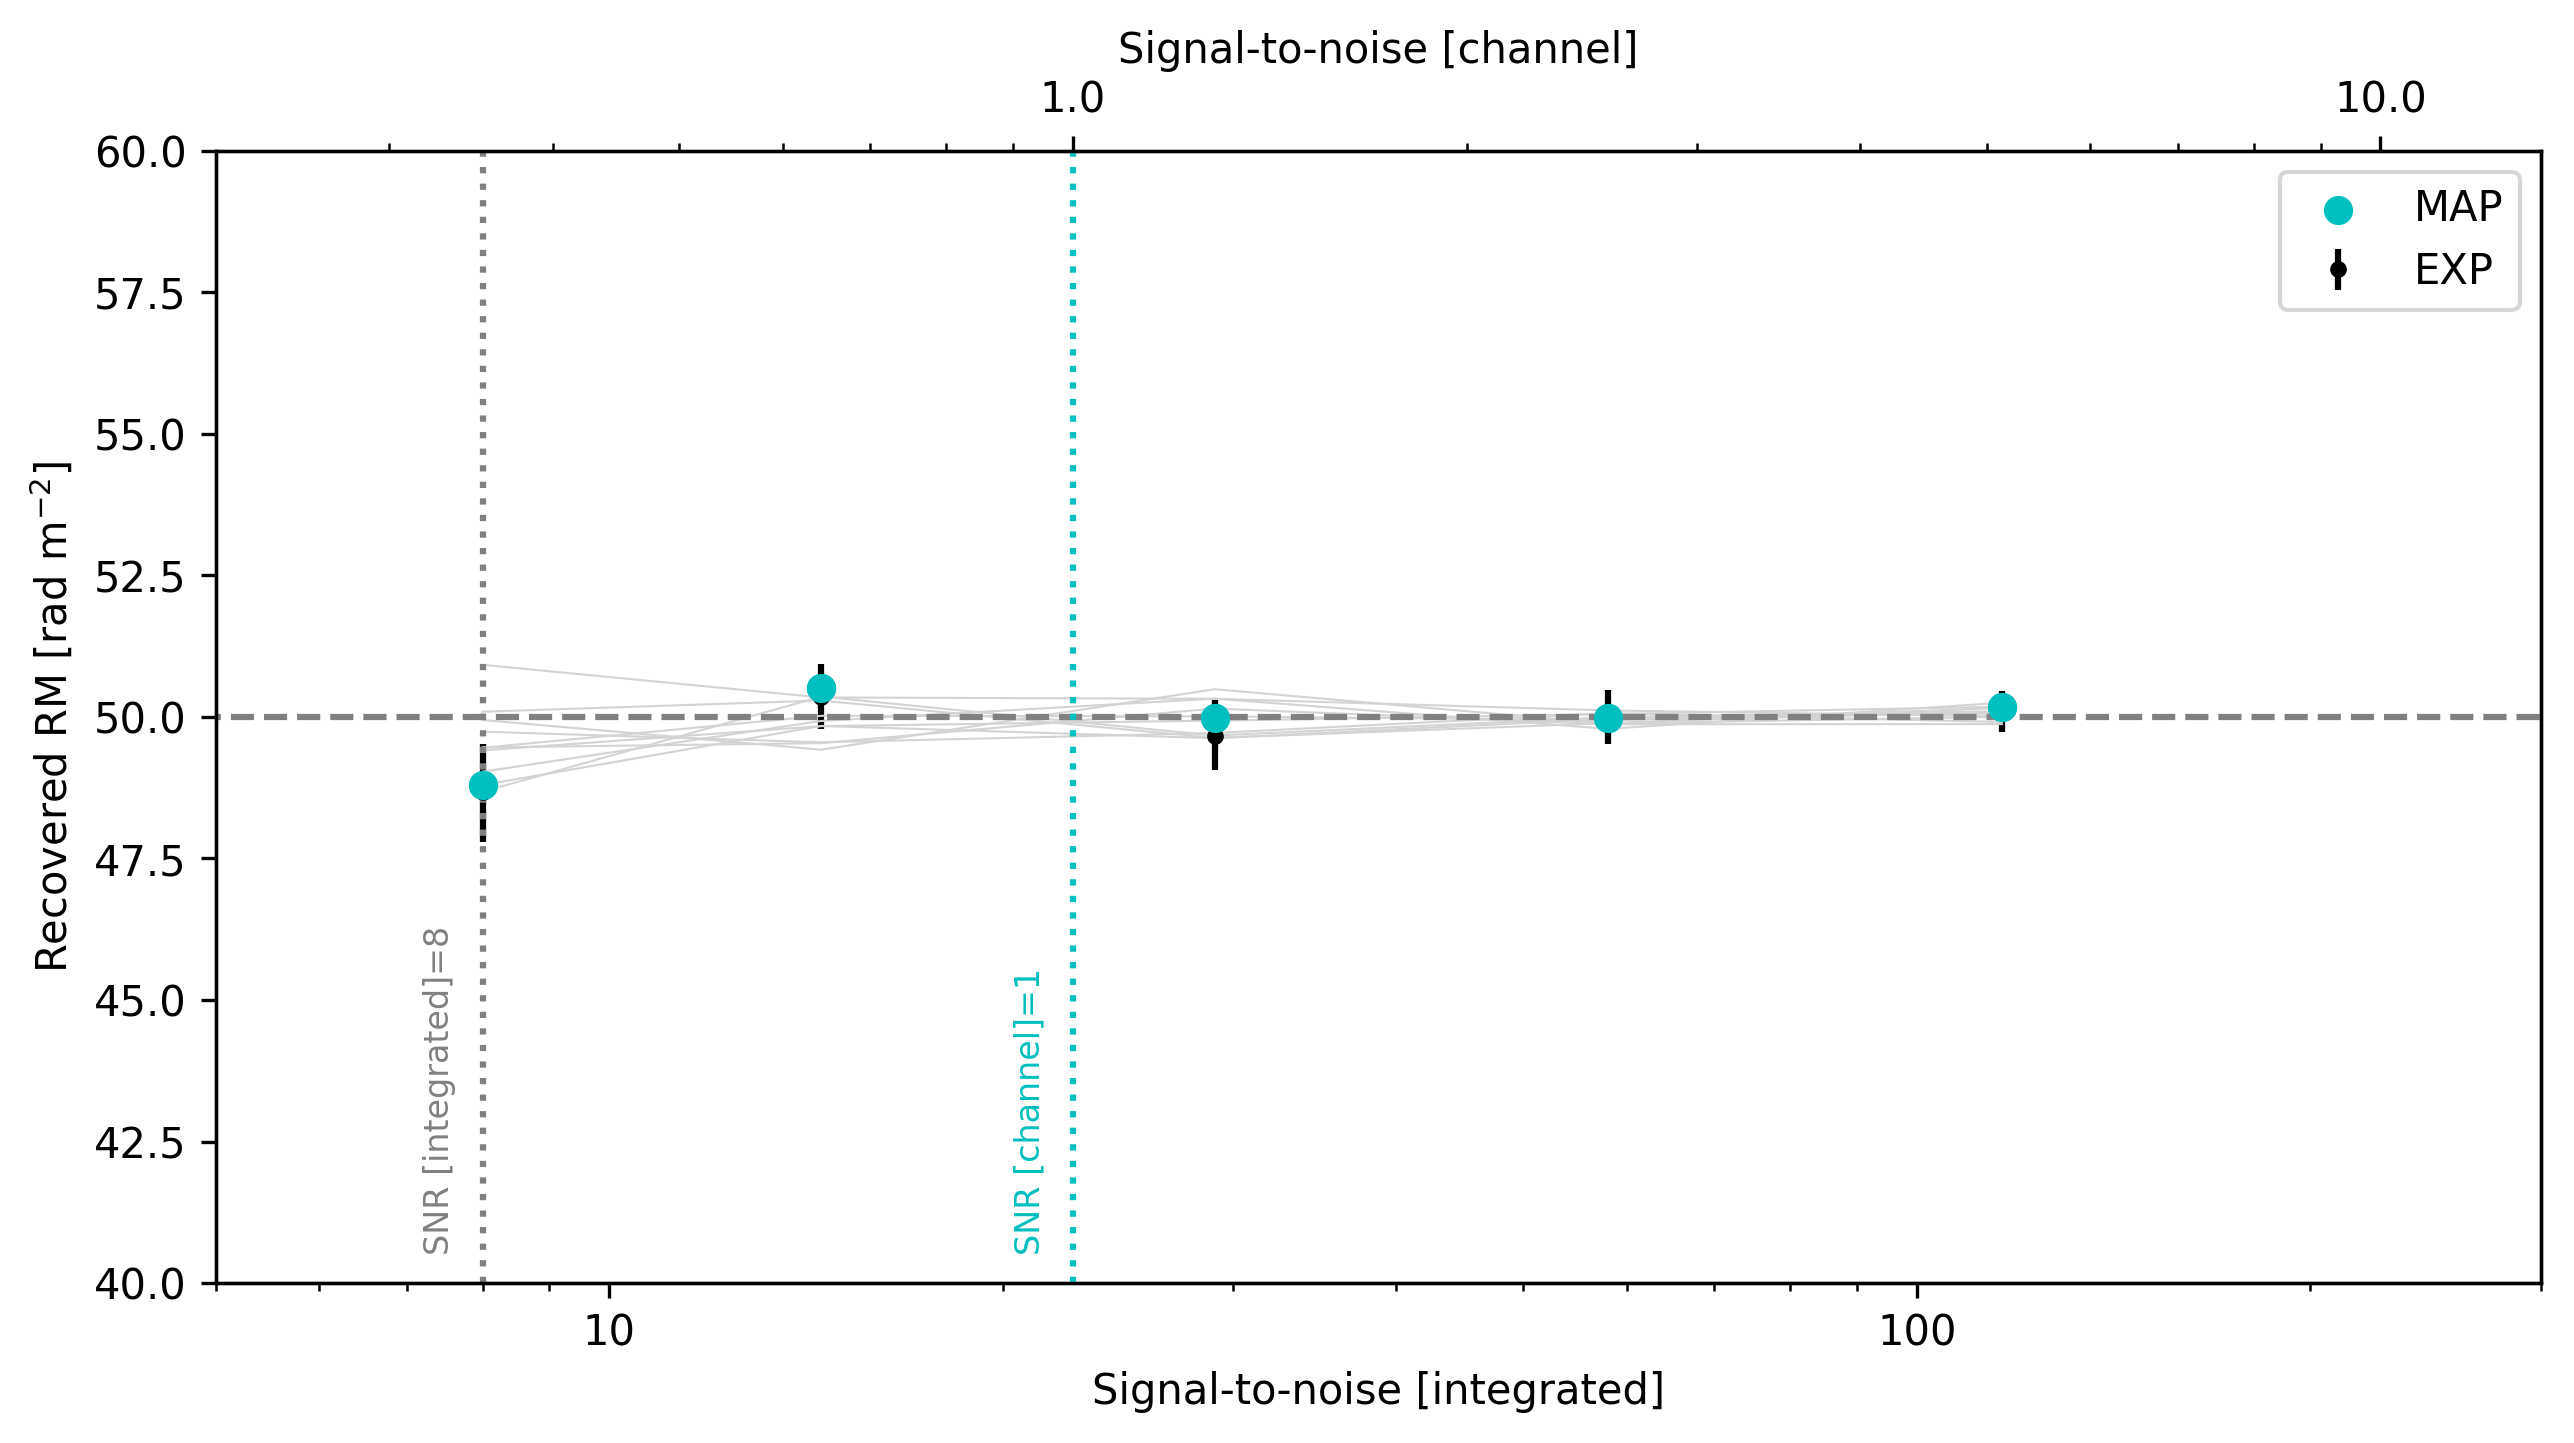
\includegraphics[width=0.9\textwidth]{./FIGURES/rm_snr.png}}
\caption{\label{fig:rm_snr} Recovered rotation measure (RM) as a function of the signal-to-noise (SNR) in the integrated polarization data for Scenario~1. Maximum likelihood RM estimates are shown as blue points, expectation RM estimates with a 68\% confidence interval are shown as black points. The true value of the RM is shown as a horizontal dashed line (grey) and the point at which the signal-to-noise in an individual frequency channel is equal to one is shown as a vertical dashed line (blue). The distribution of equivalent expectation values for ten different noise realisations are shown as light grey lines.}
\end{figure*}



\section{Performance considerations for surveys}
\label{sec:joedata}

We now extend the application to simulated data to a large data set, such as might be recovered from a MeerKAT observation of a survey field. We use a simulated data set containing Stokes~Q and Stokes~U data for 10,000 Faraday thin sources. Observational parameters are matched to those of the MeerKAT telescope, one of the precursor arrays of the Square Kilometre Array (SKA) \citep{5136190, 2009IEEEP..97.1522J}. The MeerKAT consists of 64 13.5\,m parabolic dishes sited in the Northern Cape province of South Africa \citep{Justin,Taylor_2017}. %(Jonas 2016, Taylor \& Jarvis 2017).

%Polarization surveys for the MIGHTEE survey [REF] are expected to be conducted in the MeerKAT mid-frequency band ($0.90 - 1.67$\,GHz) using 135 frequency channels across the band. This results in a channel width of $\delta\nu \approx 6$\,MHz. The relevant parameters of the MeerKAT for this work are as shown in Table~\ref{tab:meerkat} .

10,000 Faraday thin sources were created with an RM taken from a uniform distribution between -100 and +100\,rad\,m$^{-2}$. Stokes~Q and U values were generated for 320 frequency channels spaced uniformly in wavelength from 0.88\,GHz to 1.68\,GHz. The intrinsic angle of polarisation for each source, $\chi_0$, was sampled randomly from a uniform distribution $[-\pi, +\pi)$.
For each frequency channel, noise was added to the Stokes~Q and U values using a normal distribution with a mean of zero and a variance of $500\mu$\,Jy\,beam$^{-1}$, equivalent to an integrated noise level of $\sim 30\mu$Jy\,beam$^{-1}$. These specifications are equivalent to the observational parameters of the MeerKAT MIGHTEE survey \citep{Taylor_2017}.

Values for Stokes~I were taken informed by the extragalactic source counts models of \cite{dezotti}. These models cover flux density values up to 1\,Jy for Star Forming Galaxies (SFGs), and up to 148.4\,Jy for Active Galactic Nuclei (AGN).

The frequency-dependence of the flux density values were simulated with a frequency dependence of
%
\begin{equation}
\label{FreqDependent}
S_{\nu} = S_{\rm 1.4\,GHz}\left(\frac{\nu}{\rm 1.4\,GHz} \right)^{-\alpha},
\end{equation}
%
where $S_\nu$ is the flux density at each frequency, $\nu$, $S_{1.4\rm{GHz}}$ is the flux density at 1.4 $\rm{GHz}$, and $\alpha$ is the spectral index, which is taken to be the canonical value of $\alpha$ = 0.7 for synchrotron radiation.

The intensity of the polarised signal $P$ is given by
%
\begin{equation}
\label{eq:PolarisedSignal}
P = \sqrt{Q^2 + U^2} = I*\Pi,
\end{equation}
%
where $Q$ and $U$ are the Stokes parameters for linear polarisation, $I$ is the total intensity Stokes parameter, and $\Pi$ is the polarisation fraction. To simulate values for $\Pi$, the following relationship was used,
%
\begin{equation}
\label{eq:StilEquation}
\log \Pi = -(0.051\pm0.004) \log S_{\rm 1.4\,GHz} + (0.388\pm0.007)
\end{equation}
%
\citep{Stil_2014}, where $\Pi_{0, {\rm med}}$ is the median percentage polarisation fraction and $S_{\rm 1.4\,GHz}$ is the 1.4\,GHz flux density in mJy.
%
\citep{Stil_2014}, where $\Pi_{0, {\rm med}}$ is the median percentage polarisation fraction and $S_{\rm 1.4\,GHz}$ is the 1.4\,GHz flux density in mJy.

%Figure \ref{fig:PolfracVsFluxDensity} shows how the polarisation fraction varies with the flux density according to Equation~\ref{eq:StilEquation}.
%
%\begin{figure}
%\centering
%\includegraphics[width=0.45\textwidth]{./FIGURES/PolfracVsFluxDensity.png}
%\caption{\label{fig:PolfracVsFluxDensity} Plot of the polarisation fraction values determined from Eq. \ref{eq:StilEquation}, which were used in simulating data here. The red line shows  Eq. \ref{eq:StilEquation} itself plotted, and the dotted blue lines show example results for 10,000 generated sources simulated in the same way as those used in the dataset uses here. This is done to provide some context and intuition regarding the relative frequency of the polarisation fraction and flux density values in the simulated data.}
%\end{figure}
%
%\begin{table}
%\caption{\label{tab:meerkat}}
%\begin{tabular}{|l|c|c|c|c|}
%\hline
%& $\Delta \lambda^2$ & $\lambda^2_{\rm min}$ & $\delta \phi$ & $|\phi_{\rm max-scale}|$ \\\hline
%$0.58 - 1.01$\,GHz & 0.179 & 0.088 & 19.35 & 35.70\\
%$0.90 - 1.67$\,GHz & 0.079 & 0.032 & 43.85 & 98.17\\
%$1.75 - 2.50$\,GHz & 0.015 & 0.014 & 230.94 & 224.40\\\hline
%\end{tabular}
%\end{table}

We randomly select 500 sources from this population with an SNR$_{\rm int}\ge8$ and $|RM|>\phi_{\rm lim}$ and use an optimised GP with the kernel specified in Equation~\ref{eq:celkernel} to recover the rotation measure for each object. We use a prior range of $\mathcal{U}(-25,+5)$ for all hyper-parameters in log space.  The distribution of recovered RM values is shown in Figure~\ref{fig:survey}, where it is compared to the known input values. It can be seen that the rotation measures are recovered with consistently good accuracy. Errors on the recovered RMs are calculated from the 68\% confidence interval on the optimised value of $\ln P$, which results in asymmetric uncertainties on the RM values. Larger uncertainties are seen for lower SNR$_{\rm int}$ samples, as also seen in Figure~\ref{fig:rm_snr}. For 500 randomly selected samples under these constraints all of the recovered RMs lie within 5$\sigma$ of the true value and $>99\%$ within 3$\sigma$. The average run time per object is 43\,seconds on a Macbook Pro with a 3.5\,GHz Intel Core i7 processor.
%
\begin{figure*}
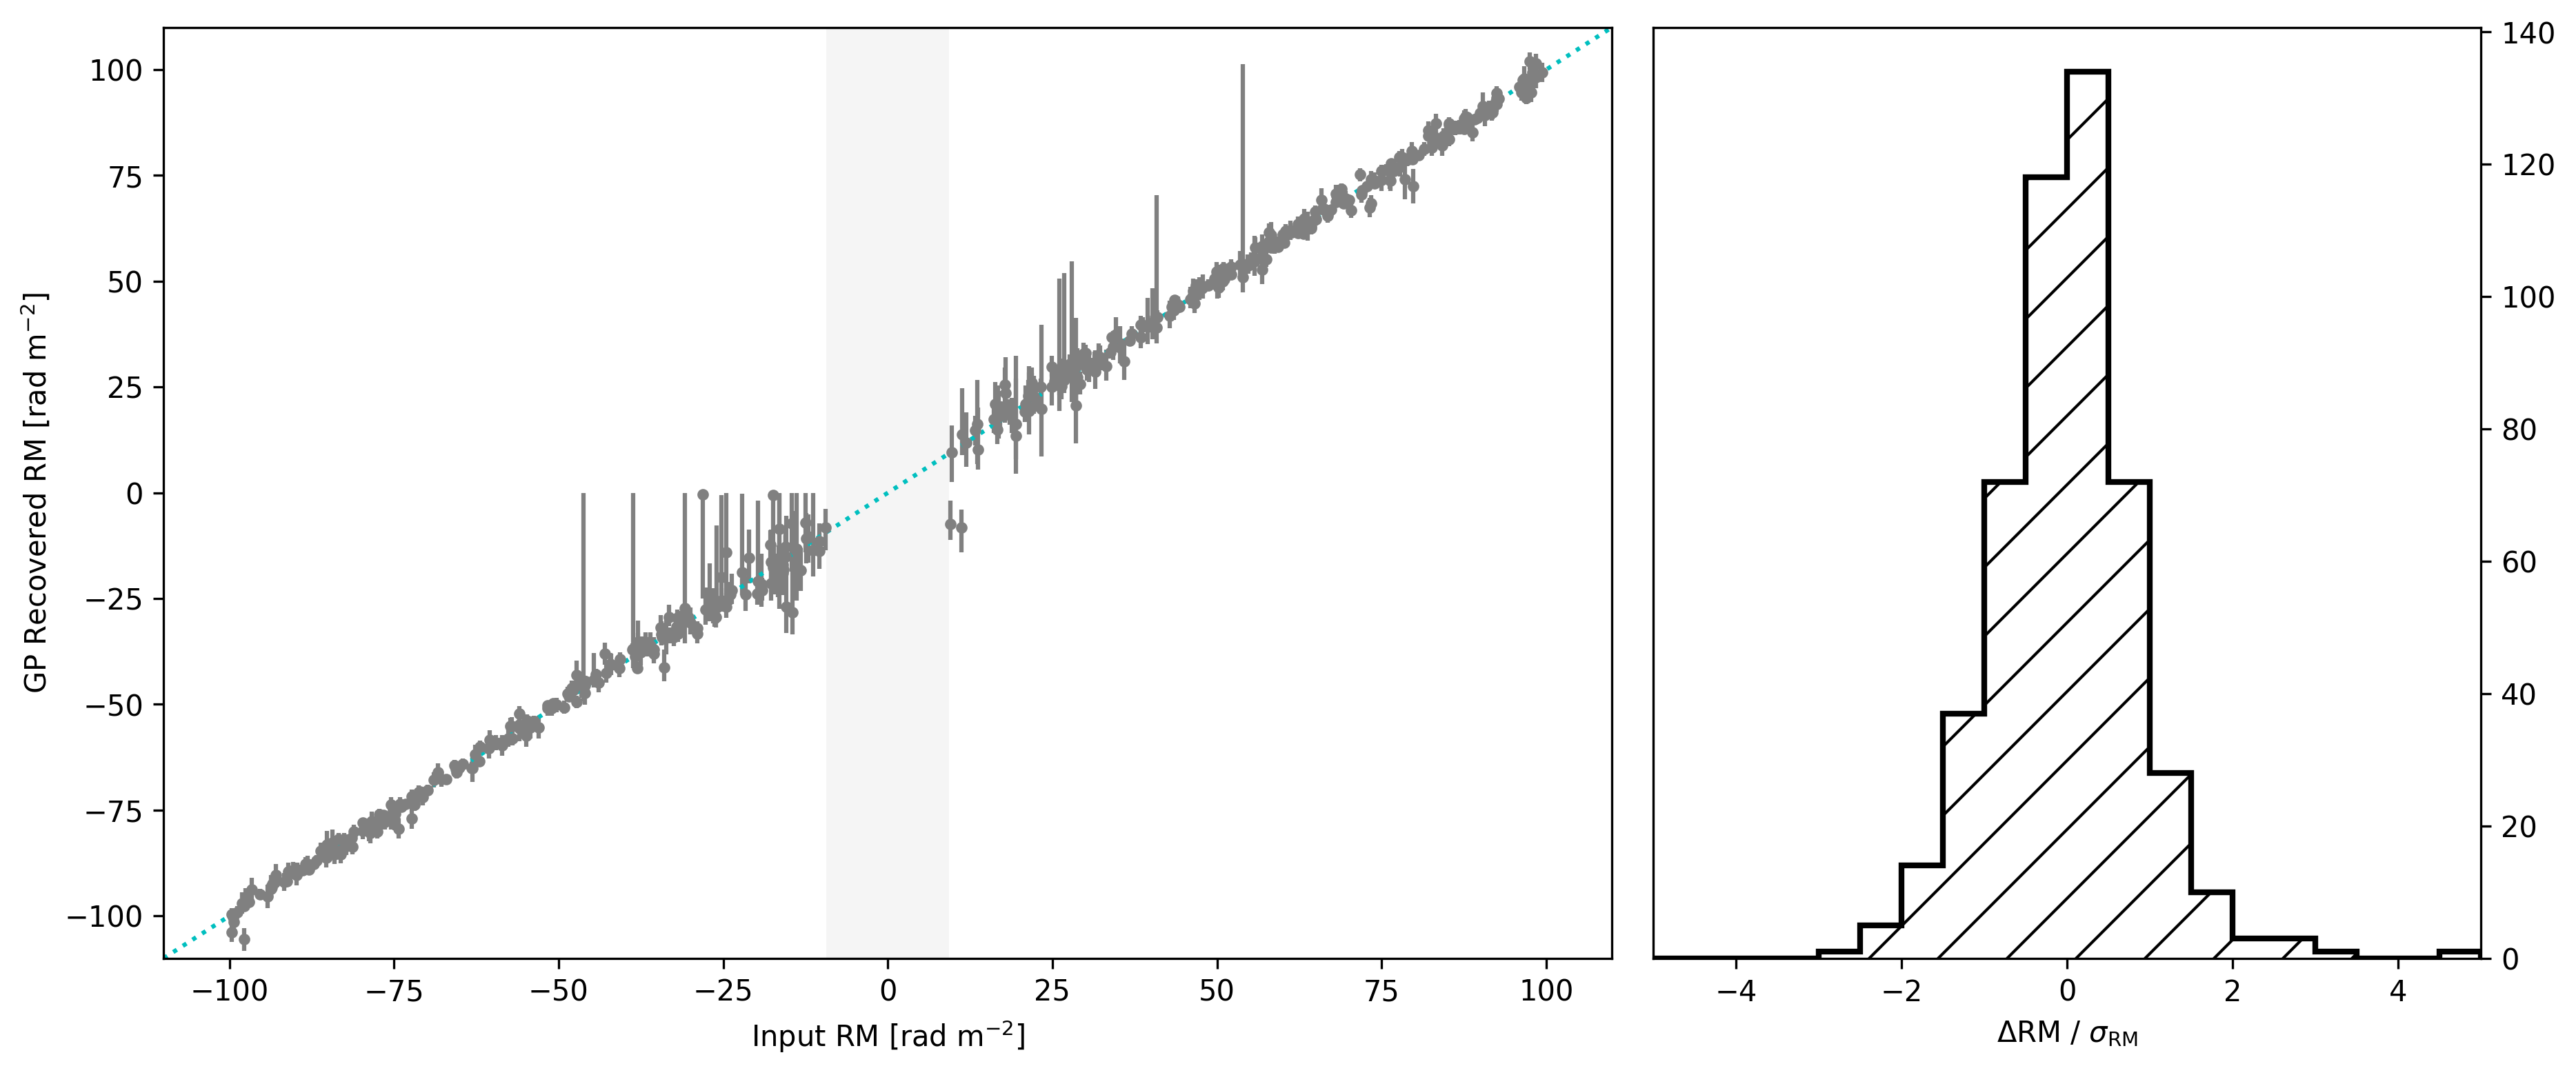
\includegraphics[width=0.9\textwidth]{./FIGURES/rm_comp.png}
\caption{\label{fig:survey} Comparison between the input RM value and the RM value recovered from the hyper-parameter of the optimised GP for each of the sources in the MeerKAT simulation. Left: input RM values against recovered RM values including uncertainties. Data have $8.06 \le$SNR$_{\rm int} \le 30.2$. The range of RMs excluded by the $\phi_{\rm lim}$ limit is shown as a shaded region. Right: Distribution of difference between input and recovered RM as a function of significance. See \S~\ref{sec:joedata} for details.}
\end{figure*}

%Data flagging for the MeerKAT in this band is expected to remove approximately $20-30\%$ of the bandwidth due to radio frequency interference from satellites.



\section{Discussion}
\label{sec:disc}

\subsection{Using GP reconstructed Faraday depth spectra}
\label{sec:usage}

Examples of Faraday depth spectra reconstructed from the optimized GP for Scenario~1 and Scenario~2 are shown in Figures~\ref{fig:flagging1}~\&~\ref{fig:flagging2}. The reconstructed Faraday depth spectra in each case (right hand column of both figures) represent the structure in the quasi-periodic component of the covariance kernel only. Although the white noise component is taken into account during the optimization, it is not appropriate to scatter the predicted values by this distribution as the white component represents the measurement noise on the original data only. As mentioned already in \S~\ref{sec:imputation}, in order to avoid over-interpretation of the reconstructed Faraday depth spectrum, features below the equivalent detection threshold in Faraday depth space should not be considered significant.

If the optimized GPM was used to predict the posterior mean only at the positions of the input data, the model could be subtracted from the data at those positions to estimate a residual, as shown in the lower panel of Figures~\ref{fig:scenario1}~\&~\ref{fig:scenario2}. This residual could then be transformed separately to the model and combined with the model reconstruction in a manner similar to that employed by the final step of the Cotton-Schwab CLEAN algorithm in synthesis imaging. We note that a GPM approach to two-dimensional image synthesis and deconvolution in radio astronomy is likely to be prohibitive in its computational complexity, as the fast separable kernels employed here are only appropriate for one-dimensional data.

\subsubsection{Recovery of Faraday thick structure}
\label{sec:thick}

As can be seen in Figure~\ref{fig:flagging2}, using an optimized GP to improve the interpretability of the Faraday depth spectrum in the case where Faraday thick structure is present can reveal these structures without the need for assuming any specific parametric model of Faraday depth a priori. Although it is not possible to recover the parameterised geometry of the thick structure from the hyper-parameters of the GP in this case, the shape is far more clearly delineated in the GP-reconstructed Faraday depth spectrum than in the spectrum calculated from the original data. This remains the case even in the presence of high degrees of RFI excision.

In principle, GPs might also be used to predict the complex polarization signal at smaller values of $\lambda^2$ than are present in the original dataset, which could be beneficial for recovering extended structure in Faraday depth space. When used to predict the behaviour of a signal outside the range of measurements, the posterior covariance of a GP will increase in response to the stationary nature of the covariance not finding any additional measurements to anchor it. This increase in covariance can be used to down-weight predicted values of the posterior mean, relative to those known with more confidence. The behaviour of the prediction will tend towards the mean function and in the general case where the mean function is assumed to be zero-valued, this is equivalent to the same logical sampling as in the original dataset; however, for spectra where Faraday thick structure are present, which have non-zero means at low-$\lambda^2$ this may artificially truncate structure. This was found to be the case here for the kernel in Equation~\ref{eq:celkernel} when used to extend $\lambda^2$-space as illustrated in Figure~\ref{fig:resampling}.

It is also important to note that structures which exist only on scales larger than that set by the measured $\lambda^2_{\rm min}$ will {\it not} be recovered by a GP model used for prediction outside the range of the original measurements. Hence this form of structure enhancement for Faraday thick structures can only be used to improve the recovery of structures which exist on scales that are already sampled in part by the original measurements. Any larger structures will not appear in the Faraday depth spectrum of the GP reconstruction, an effect analogous to flux loss in synthesis imaging for radio interferometry.


\subsubsection{Polarization leakage}
\label{sec:leakage}

In the scenarios considered here, we have assumed a zero-valued mean function. In the absence of instrumental leakage, this assumption is valid for modelling Faraday rotation; however, the presence of residual instrumental leakage can result in a non-zero offset in both Stokes~Q and Stokes~U. The inclusion of such a constant offset as a free parameter (separately for Q and U) in the optimization process is straightforward to implement and requires only very minor changes to be made in the calculation of the posterior mean. However, for some telescopes with wide bandwidths, polarization leakage can be frequency-dependent and consequently modelling it as a constant offset will not be sufficient. In this case there is potential for confusion between the leakage term and covariate behaviour in the complex polarization; as can be seen in Figure~\ref{fig:scenario2}, smoothly varying systematic changes in amplitude can be modelled perfectly well using stationary kernels.

\subsection{Faraday Challenge}
\label{sec:challenges}

%\cite{Sun_2015} ran a data challenge that compared Faraday depth and QU-fitting algorithms across a set of common Faraday depth models.
%

%
In order to evaluate the performance of the GP approach against other methods in the literature we use the 17 models from the Faraday challenge of \cite{Sun_2015}. These models include examples of single Faraday thin objects, multiple (two) Faraday thin objects, and combinations of  Faraday thick and Faraday thin objects. While the GP approach can only determine RM values in the case of single Faraday thin models, we can use the model evaluation metrics to compare the predicted Faraday depth spectra in all cases. For this purpose we use the kernel from Equation~10 for all test data sets with priors as listed in Table~\ref{tab:priors}. All evaluations are made on models with SNR$_{\rm int}$=32, as in \cite{Sun_2015}.

%The parameters for each model are listed in Table~\ref{tab:challenge} and we use the same method as described in \S~\ref{sec: } with hyper-parameter priors as given in Table~\ref{tab:challengepriors}.
The reduced $\chi^2$ for parametric models described in \cite{Sun_2015} is roughly equivalent to the standardized mean squared error (SMSE). For an optimised GP, the SMSE is defined as
%
\begin{equation}
SMSE = \frac{1}{N}\left[ \frac{(P - P_{\ast})^2}{\sigma_{\rm n}^2}  \right],
\end{equation}
%
where $P_{\ast}$ is the posterior mean prediction of complex polarization from the optimized GP, $P$ is the input complex polarization, and $\sigma_{\rm n}^2$ is the variance of the white noise on the input data. In order to account for the independence of the white noise between Stokes~Q and U we set $N=600$. The difference between the SMSE and the $\chi^2_{\rm r}$ used by \cite{Sun_2015} is the normalisation, which instead uses $N-K$ in the denominator where $K$ is the number of parameters. Although the GP used here is not strictly parametric, we calculate this quantity using $K=4$ to represent the number of hyper-parameters in our model.

Since the GP optimisation method produces a full predictive distribution at the position of each test sample, we also calculate the mean standardised log likelihood as a measure of performance \citep{3569}. The negative log-likelihood for the GP is given by,
%
\begin{equation}
\label{eq:logl}
-\log L^{\ast} = \frac{1}{2}\log(2\pi \sigma_{\ast}) + \frac{(P - P_{\ast})^2}{2\sigma_{\ast}^2},
\end{equation}
%
where $D$ are the input training data, $P$ are the input polarization data, $P_{\ast}$ are the GP reconstructed polarization data, and $\sigma_{\ast}^2$ is the variance of the GP reconstruction, defined in Equation~\ref{eq:gpvar}.
We standardise this loss by subtracting the equivalent loss as calculated using a model that predicts using a simple Gaussian with the mean and variance of the input data. The individual performance metrics for each model in the Faraday challenge are listed in Appendix~\ref{app:challenge}.

The median of the reduced chi-squared statistic recovered from our model, $\chi^2_{\rm r} = 0.99$, is in good agreement with the expected optimum value of $1.00\pm0.02$ from Sun et~al. (2014). Results for both the SMSE and $\chi_{\rm r}^2$ across all 17 test models, evaluated using SNR=32 as in \cite{Sun_2015}, are shown in Figure~\ref{fig:sunmetrics}. By comparison to Figure~3 in that work it can be seen that the GP $\chi_{\rm r}^2$ has a median value comparable to that of the three best performing methods in that work, each of which use QU-fitting approaches. Furthermore, it can also be seen that the distribution of $\chi_{\rm r}^2$ for the GP method is significantly narrower than those methods, each of which has a 68\% confidence interval that extends to values larger than $\chi_{\rm r}^2=1.1$.
%
\begin{figure}
    \centering
    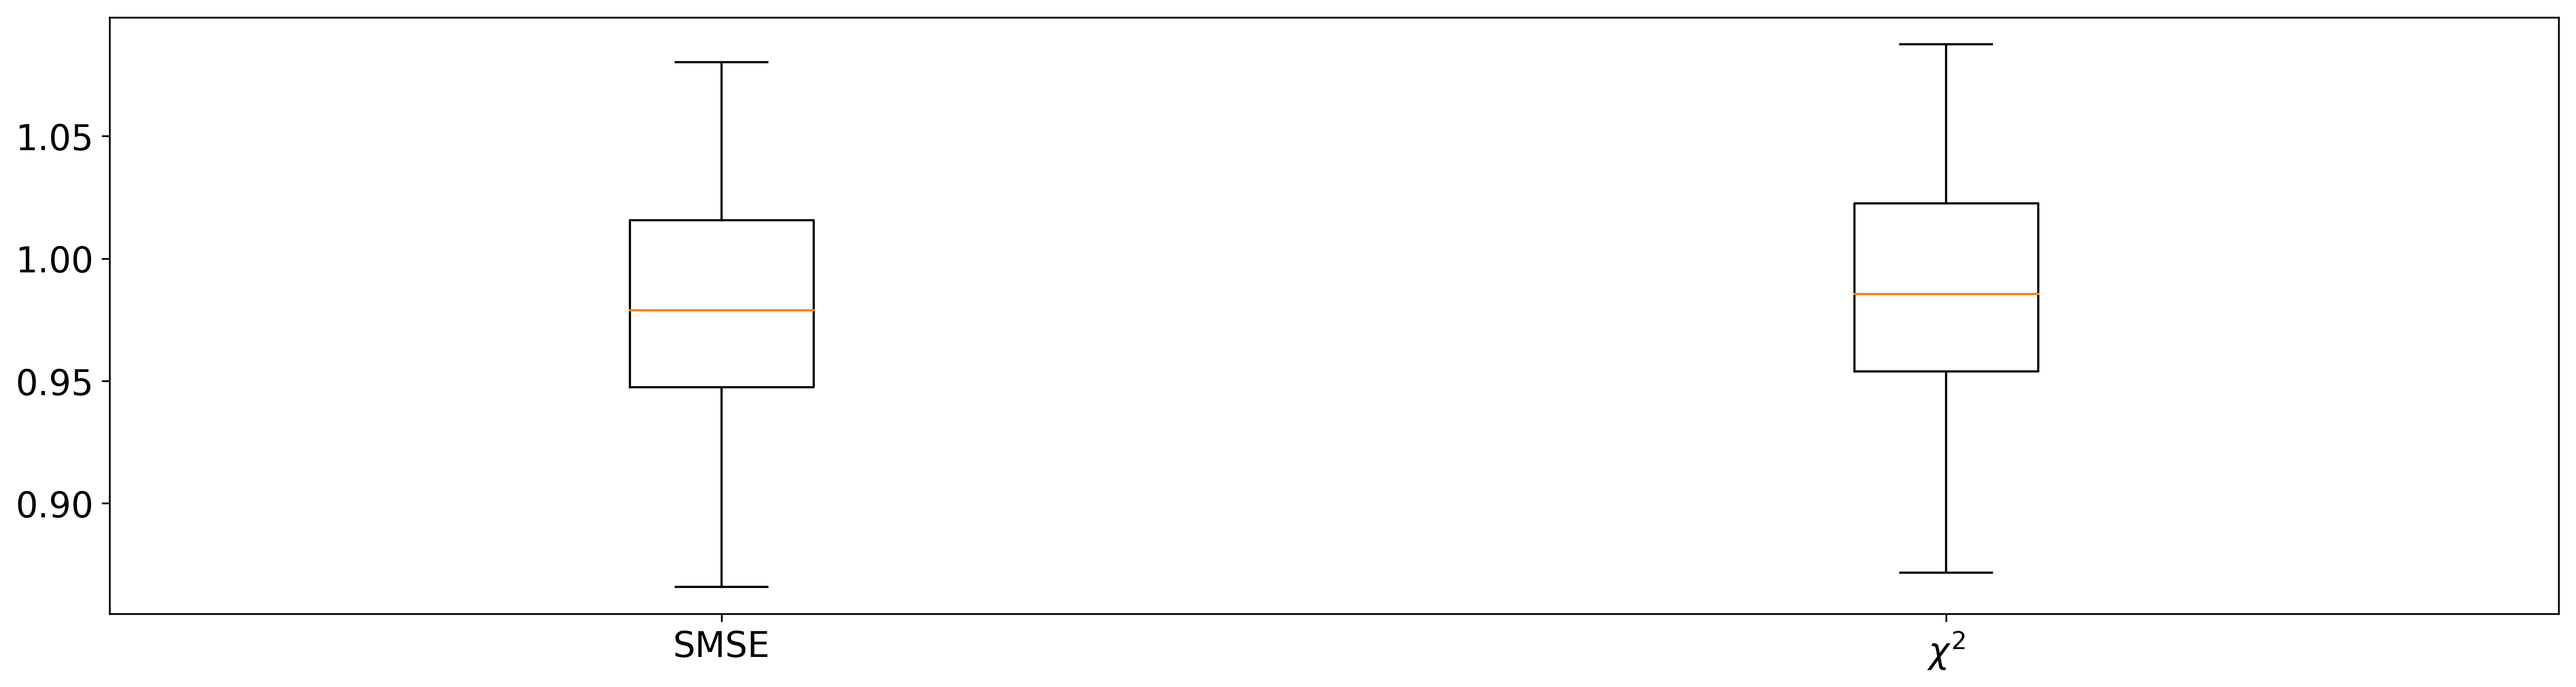
\includegraphics[width=0.45\textwidth]{./FIGURES/smse.png}
    \caption{Box-and-whisker plots for figures of merit over all 17 tests. The boxes show the first, the second (median), and the third quartile, and the ends of the whiskers show the minimum and maximum values.}
    \label{fig:sunmetrics}
\end{figure}

%\cite{Sun_2015} also evaluated the performance of algorithm outputs using a comparison between the weighted average of Faraday depth between the input model and the prediction, denoted here as $\Delta RM_{\rm wtd}$, where
%
%\begin{equation}
%RM_{\rm wtd}(F) = \frac{\sum_{i}{|F_i|\phi_i}}{\sum_{i}{|F_i|}},
%\end{equation}
%
%where $|F_i|$ is the magnitude of the Faraday depth spectrum for Faraday thin model component $i$ and $\phi_i$ is the Faraday depth of that component. The quantity, $RM_{\rm wtd}$, is a strong function of the range of Faraday depth in the calculated spectrum and should not be used without differencing against a reference spectrum, e.g. $RM_{\rm wtd}(F_{\rm test} - F_{\rm model})$.

\subsection{Alternative kernels}
\label{sec:infocrit}

For a given regression problem, there are an infinite number of models that can be used. As such, it is usually not feasible to test all possible models. In this work so far we have used the GP kernel defined in Equation~\ref{eq:celkernel}; here we consider the use of alternative kernels. We denote our original kernel as as ``3-HP" and we compare it to (i) the quasi-periodic kernel used by \cite{celerite} to model stellar variability, and (ii) a hybrid kernel including a second squared-exponential term.

In \cite{celerite}, the period of rotation of a star was determined by extracting the optimised $P$ hyper-parameter, analogous to our use of $P$ to estimate the rotation measure of a Faraday thin source. The stellar variability kernel from \cite{celerite} is also built using the {\tt celerite} library and has the form,
%
\begin{equation}
\label{eq:4hpkernel}
k(x_i,x_j)=\frac{B}{1+C}\,{\rm e}^{-A|x_i - x_j|}\left[\cos\left(\frac{2\pi|x_i - x_j|}{P}\right) + (1+C)\right],
\end{equation}
%
where $A$, $B$, $C$ and $P$ are hyper-parameters. We denote this kernel as ``4-HP".

The hybrid kernel, denoted here as ``5-HP", has the form,
%
\begin{equation}
\label{eq:5hpkernel}
k(x_i,x_j)=h_1\,{\rm e}^{-c_1|x_i - x_j|}\cos\left(\frac{2\pi|x_i - x_j|}{P}\right) + h_2\,{\rm e}^{-c_2|x_i - x_j|},
\end{equation}
%
where $h_1$, $c_1$, $P$, $h_2$ and $c_2$ are hyper-parameters. Both the 4-HP and 5-HP kernels have an extra term which is intended to model smoothly varying non-periodic behaviour such as that which might arise from Faraday thick components along the line of sight.

Although different methods of evaluating competing models have been developed, the computational complexity involved in applying them limits their applicability. To overcome this limitation, easier-to-use approximate methods are commonly used to compare the performance of two or more models. These include the Bayesian Information Criterion (BIC), the Akaike Information Criterion (AIC) and the corrected Akaike Information Criterion (AICc). These information criteria are designed to evaluate the amount of information lost by a particular model. The model that loses the least information, i.e. has the lowest valued information criterion, is considered to be the preferred model.

\cite{burnham} suggest that the  BIC is  a powerful model selection tool when the `true' model is in the set of test models; however, in the case of empirical data where the true model is unlikely to be known a priori the AIC is considered to be a more appropriate criterion. Furthermore, the \emph{corrected} AIC places a stronger complexity penalty on models used with finite data series than the original AIC. In the case of small sample sizes it is considered to be more appropriate and accurate for finding the preferred model. However, \cite{kassrafferty} suggest that the AIC should only be used in situations where the prior distribution is similar to that of the likelihood and that when this isn't the case and the prior is significantly less informative than the likelihood then the BIC will favour simpler models than the AIC.

For each sample dataset we optimize the hyper-parameters for each of the three kernels using the method described in \S~\ref{sec:optimization} and use these values to compute the Bayesian Information Criteria \citep[BIC;][]{1978AnSta...6..461S},
%
\begin{equation}
{\rm BIC} = -2 \log L^\ast + K \log N,
\end{equation}
%
the Akaike Information Criterion \citep[AIC;][]{AIC},
%
\begin{equation}
{\rm AIC} = 2 K - 2\log L^\ast,
\end{equation}
%
and the corrected AIC \citep[AICc;][]{AICc},
%
\begin{equation}
{\rm AICc} = {\rm AIC} + \frac{2K(K+1)}{N - K - 1},
\end{equation}
%
where $\log L^\ast$ is given by Equation~\ref{eq:logl}, $K$ is the number of hyper-parameters, and $N=600$ is the number of data points.

We calculate the median value and inter-quartile range for each of the three information criteria from ten different noise realisations with SNR$_{\rm int}$=32.
%Examples of these values are shown in Table~\ref{tab:icthin} for the models with only one Faraday thin component, and are continued in Appendix~\ref{app:ic} for the other fourteen models.
%
The goodness of fit statistics for the Faraday challenge models using the two alternative kernels are $\chi^2_{\rm r} = 0.98$ for the 4-HP model, and $\chi^2_{\rm r} = 0.97$ for the 5-HP model.

The median values of the information criteria suggest a preference for the HP-4 kernel in the case of single Faraday thin component models, a preference for the HP-5 kernel in the case of double Faraday thin models, and a preference for the HP-3 kernel in the case of Faraday thick models. However, we note that these are modal preferences and no model type shows a unanimous preference for a particular kernel. Indeed, although ranking the three kernels using the median value of the information criteria for each data set may nominally show a preference for one kernel above others, the overlapping inter-quartile ranges for most models suggest that there is in fact no clear preference. The only model where one kernel is significantly preferred is Model 1, where the inter-quartile range of the HP-4 kernel is outside the inter-quartile range of both other kernels, see Figure~\ref{fig:model1bic}. We also see no difference in the median ranking across the three information criteria, which is perhaps unsurprising given that $N \gg K$ in all cases. Furthermore, as noted by \cite{biccomp}, information criteria comparisons are appropriate only for data sets with the same number of measurement samples, and we emphasise that the kernel comparison presented here is for the specifications of the test sets in the \cite{Sun_2015} Faraday challenge.
%
\begin{figure}
    \centering
    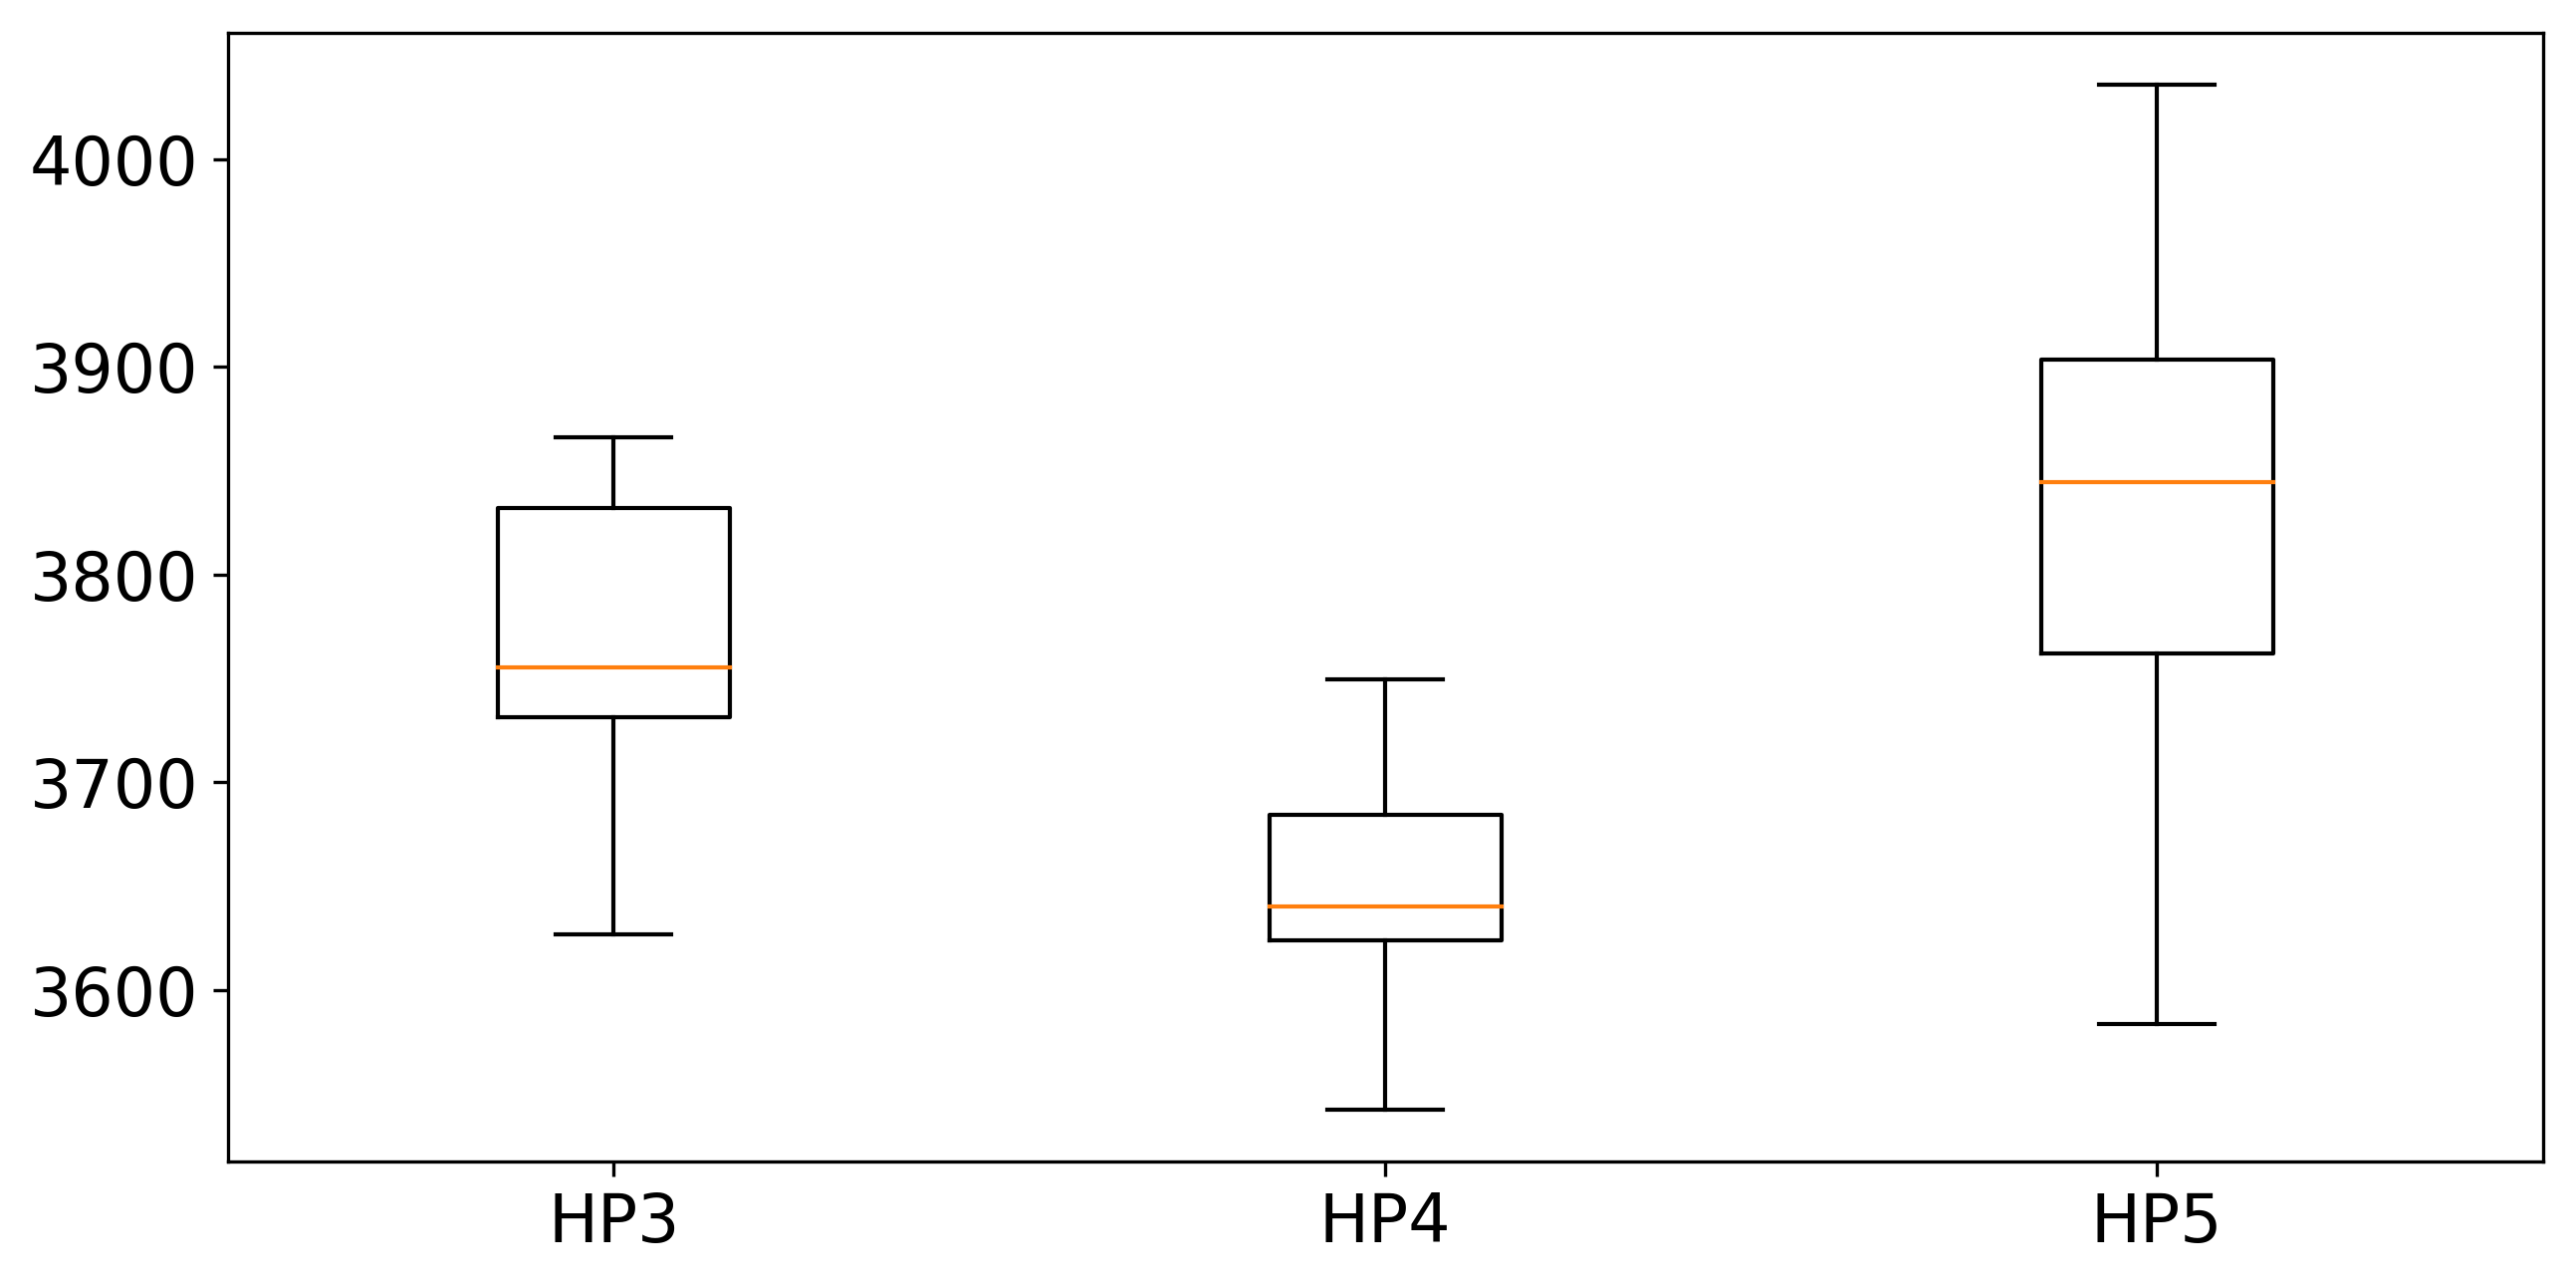
\includegraphics[width=0.45\textwidth]{./FIGURES/model0_info.png}
    \caption{Box-and-whisker plots for BIC values derived from each of the 3 kernels using 10 noise realisations of Model 1 from \protect\cite{Sun_2015}. The boxes show the first, the second (median), and the third quartile, and the ends of the whiskers show the minimum and maximum values.}
    \label{fig:model1bic}
\end{figure}



\section{Conclusions}
\label{sec:conclusions}

In this work we suggest that Gaussian Process Modelling (GPM) may be a flexible alternative to traditional QU-fitting methods as it does not rely on an exact parameterised physical model, or set of models, to be known a priori and is therefore suitable for situations where some prior knowledge of the form of the signal is understood, but the exact line of sight structure is imperfectly known. This is often the case for Faraday depth analysis. With regard to this, we have shown that even simple GPM covariance kernels may be used to impute data reliably for complex lines of sight and improve the interpretability of their resulting Faraday depth spectra.

We have demonstrated the applicability of GPM for improved recovery of structure in Faraday depth spectra. We have shown that these improvements include the reduction of sidelobe contamination in Faraday depth spectra through imputation of missing data when RFI flagging causes significant losses, even in the case where significant portions of the original data set are lost. We have also illustrated the benefits of using GPM to re-sample complex polarization data onto regular spacings in $\lambda^2$-space as an alternative to currently used re-gridding methods. We have shown that these applications in combination can provide an improved representation of Faraday thick structure in Faraday depth spectra.

We have shown that under certain circumstances the hyper-parameters of the periodic covariance kernel can be used to recover rotation measure values for Faraday thin sources and that this hyper-parameter can also be physically meaningful in a more limited way for complex lines of sight. We have presented a method to calculate the range of RM over which this method is applicable for different telescopes and/or data sets and we have demonstrated that within this range RM recovery from GP hyper-parameters is robust to typical detection thresholds.


We have discussed the limitations in the interpretation of GPM reconstructed Faraday depth spectra, highlighted situations in which GPM is not an appropriate solution and presented a quantitative method for determining a threshold above which Faraday structure can be safely considered significant when reconstructed using an optimised GP fitted to noisy data.

We have evaluated the GP reconstruction proposed here against other methods in the literature and have shown that it has a performance equivalent to other QU-fitting methods and furthermore that the variance in results from the GP approach is smaller than seen from those methods. Using the same test data we have quantitatively confirmed our assertion that even complex Faraday structure can be re-constructed equivalently well using a comparatively simple covariance kernel.


\section*{Acknowledgements}

SWN acknowledges support from the UK Newton Fund via the Science \& Technology Facilities Council (STFC) through the Development in Africa with Radio Astronomy (DARA) Big Data project. AMS gratefully acknowledges support from an Alan Turing Institute AI fellowship. JH acknowledges support from the UK Science \& Technology Facilities Council (STFC). MC acknowledges support from CONICYT PFCHA/DOCTORADO BECAS CHILE/2018-72190574.

%%%%%%%%%%%%%%%%%%%%%%%%%%%%%%%%%%%%%%%%%%%%%%%%%%

%%%%%%%%%%%%%%%%%%%% REFERENCES %%%%%%%%%%%%%%%%%%

% The best way to enter references is to use BibTeX:

\bibliographystyle{mnras}
\bibliography{GPM} % if your bibtex file is called example.bib


% Alternatively you could enter them by hand, like this:
% This method is tedious and prone to error if you have lots of references
%\begin{thebibliography}{99}
%\bibitem[\protect\citeauthoryear{Author}{2012}]{Author2012}
%Author A.~N., 2013, Journal of Improbable Astronomy, 1, 1
%\bibitem[\protect\citeauthoryear{Others}{2013}]{Others2013}
%Others S., 2012, Journal of Interesting Stuff, 17, 198
%\end{thebibliography}

%%%%%%%%%%%%%%%%%%%%%%%%%%%%%%%%%%%%%%%%%%%%%%%%%%

%%%%%%%%%%%%%%%%% APPENDICES %%%%%%%%%%%%%%%%%%%%%

\appendix

\section{Faraday Challenge Models}
\label{app:challenge}
%
\newcommand\Tstrut{\rule{0pt}{2.6ex}}       % top strut
\newcommand\Bstrut{\rule[-1.1ex]{0pt}{0pt}} % bottom strut
%
 \begin{table*}
\caption{}
\begin{tabular}{@{\extracolsep{4pt}}|l|c|c|c|c|c|c|c|c|c|c|c|c|@{}}
\hline
 & \multicolumn{9}{c}{Input Parameters} &  \multicolumn{3}{c}{Evaluation Metrics} \\
  \cline{2-10}  \cline{11-13} \Tstrut
 & $p_1$ & $\phi_1$ & $\chi_1$ & $p_2$ & $\phi_2$ & $\chi_2$ & $p_0$ & $\phi_{\rm c}$ & $\phi_{\rm s}$ & $\chi^2_r$ & SMSE & MSLL  \\
 & $\%$ & rad\,m$^{-2}$ & deg & $\%$ & rad\,m$^{-2}$ & deg & $\%$ & rad\,m$^{-2}$ & rad\,m$^{-2}$ & & &  \\\hline
Model 1 & 100.00 & 500.10 & 40.00 & $-$ & $-$ & $-$ & $-$ & $-$ & $-$ & 1.01 & 1.00 & -1.37  \\
Model 2 & 100.00 & 49.38 & 60.00 & $-$ & $-$ & $-$ & $-$ & $-$ & $-$ & 0.92 & 0.91 & -0.95   \\
Model 3 & 100.00 & 4.96 & 60.00 &  $-$ &  $-$ &  $-$ & $-$ & $-$ & $-$   & 1.00 & 1.00 & -0.47  \\
Model 4 & 25.00 & $-37.84$ & 0.00 & 16.70 & 103.18 & $-36.00$ & $-$ & $-$ & $-$  & 0.95 & 0.95 & -1.00  \\
Model 5 & 25.00 & $-37.84$ & $-40.00$ & 24.00 & 5.05 & $-40.00$ & $-$ & $-$ & $-$  & 0.98 & 0.97 & -0.57   \\
Model 6 & 25.00 & $-37.84$ & $-40.00$ & 9.00 & 5.05 & $-40.00$ & $-$ & $-$ & $-$  & 1.04 &  1.03 & -0.92   \\
Model 7 & 25.00 & $-44.55$ & 0.00 & 16.70 & 37.50 & 72.00 & $-$ & $-$ & $-$  & 0.90 & 0.89 & -0.58   \\
Model 8 & 25.00 & 232.56 & 40.00 & 9.00 & 192.70 & 40.00 &&&  & 0.94 & 0.93 & -1.31 \\
Model 9 & 25.00 & $-37.83$ & $-40.00$ & 16.50 & 5.05 & 140.00 & $-$ & $-$ & $-$  & 0.97 & 0.96 & -0.71  \\
Model 10 & 25.00 & $-37.84$ & 0.00 & 9.00 & 103.00 & $-36.00$ & $-$ & $-$ & $-$   & 1.00 &  0.99 & -1.02  \\
Model 11 & 25.00 & 149.50 & $40.00$ & 23.75 & 163.50 & $-68.00$ & $-$ & $-$ & $-$   & 0.87 & 0.87 & -1.34 \\
Model 12 & 25.00 & $-232.56$ & 0.00 & 9.00 & $-50.10$ & 72.00 & $-$ & $-$ & $-$  & 0.99 & 0.98 & -1.31 \\
Model 13 & 25.00 & $-44.55$ & 0.00 & 24.00 & 37.54 & 72.00 & $-$ & $-$ & $-$   & 0.98 & 0.97 & -0.61 \\
Model 14 &  $-$ & $-$ & $-$ & $-$ & $-$ & $-$ & 1.90 & $-136.98$ & 50.00  & 0.82 & 0.82 & -1.44  \\
Model 15 & 1.80 & $-240.22$ & $-36.00$ & $-$ & $-$ & $-$ & 1.90 & $-250.17$ & 50.00  & 1.09 & 1.09 & -1.38 \\
Model 16 & $-$ & $-$ & $-$ & $-$ & $-$ & $-$ & 1.90 & $-136.98$ & 25.00  & 0.86 & 0.86 & -1.45 \\
Model 17 & 1.80 & $-240.00$ & $-36.00$ & $-$ & $-$ & $-$ & 1.90 & $-250.17$ & 25.00  & 0.93 & 0.92 & -1.31  \\\hline
\end{tabular}
\label{tab:challenge}
\end{table*}

\section{Information Criteria}
\label{app:ic}

\begin{table*}
\caption{Information criteria comparison for the \protect\cite{Sun_2015} single component Faraday thin challenge models.}
    \centering
    \begin{tabular}{@{\extracolsep{3pt}}lccccccccc@{}}
    \hline
     & \multicolumn{3}{c}{\textbf{BIC}} & \multicolumn{3}{c}{\textbf{AIC}} & \multicolumn{3}{c}{\textbf{AICc}} \\
     \cline{2-4} \cline{5-7} \cline{8-10} \\
     & HP3 & HP4 & HP5 & HP3 & HP4 & HP5 & HP3 & HP4 & HP5 \\\hline
    \textbf{Model 1} & & & & & & & & & \\
    \emph{Median} & 3755.15 & 3640.21 & 3844.46 & 3737.56 & 3618.23 & 3818.08 & 3737.50 & 3618.12 & 3817.94 \\
    \emph{IQR} & 100.50 & 60.49 & 141.18 & 100.50 & 60.49 & 141.18 & 100.50 & 60.49 & 141.18 \\
    \emph{Median Rank} & 2 & \textbf{1} & 3 & 2 & \textbf{1} & 3 & 2 & \textbf{1} & 3 \\\hline
    \textbf{Model 2} & & & & & & & & & \\
    \emph{Median} & 3470.12 & 3402.59 & 3586.46 & 3452.53 & 3380.61 & 3560.08 & 3452.46 & 3380.51 & 3559.93 \\
    \emph{IQR} & 176.85 & 140.70 & 201.36 & 176.85 & 140.70 & 201.36 & 176.85 & 140.70 & 201.36 \\
    \emph{Median Rank} & 2 & \textbf{1} & 3 & 2 & \textbf{1} & 3 & 2 & \textbf{1} & 3 \\\hline
    \textbf{Model 3} & & & & & & & & & \\
    \emph{Median} & 1747.28 & 1773.87 & 1784.08 &1729.69 & 1751.88 & 1757.70 & 1729.62 & 1751.78 & 1757.56 \\
    \emph{IQR} & 24.82 & 25.29 & 40.32 & 24.82 & 25.29 & 40.32 & 24.82 & 25.29 & 40.32 \\
    \emph{Median Rank} & \textbf{1} & 2 & 3 & \textbf{1} & 2 & 3 & \textbf{1} & 2 & 3 \\\hline
    \end{tabular}
 \label{tab:icthin}
\end{table*}

\begin{table*}
\caption{Information criteria comparison for the \protect\cite{Sun_2015} two component Faraday thin challenge models.}
    \centering
    \begin{tabular}{@{\extracolsep{3pt}}lccccccccc@{}}
    \hline
     & \multicolumn{3}{c}{\textbf{BIC}} & \multicolumn{3}{c}{\textbf{AIC}} & \multicolumn{3}{c}{\textbf{AICc}} \\
     \cline{2-4} \cline{5-7} \cline{8-10} \\
     & HP3 & HP4 & HP5 & HP3 & HP4 & HP5 & HP3 & HP4 & HP5 \\\hline
    \textbf{Model 4} & & & & & & & & & \\
    \emph{Median} & 4277.15 & 4271.52 & 4240.80 & 4259.56 & 4249.53 & 4214.42 & 4259.49 & 4249.43 & 4214.28 \\
    \emph{IQR} & 159.35 & 129.16 & 310.82 & 159.35 & 129.16 & 310.82 & 1159.35 & 129.16 & 310.82 \\
    \emph{Median Rank} & 3 & 2 & \textbf{1} & 3 & 2 & \textbf{1} & 3 & 2 & \textbf{1} \\\hline
    \textbf{Model 5} & & & & & & & & & \\
    \emph{Median} & 2243.48 & 2227.26 & 2177.76 & 2225.89 & 2205.27 & 2151.37 & 2225.82 & 2205.17 & 2151.23 \\
    \emph{IQR} & 78.90 & 47.88 & 183.96 & 78.90 & 47.88 & 183.96 & 78.90 & 47.88 & 183.96 \\
    \emph{Median Rank} & 3 & 2 & \textbf{1} & 3 & 2 & \textbf{1} & 3 & 2 & \textbf{1} \\\hline
    \textbf{Model 6} & & & & & & & & & \\
    \emph{Median} & 2607.97 & 2647.48 & 2609.77 & 2590.38 & 2625.50 & 2583.39 & 2590.31 & 2625.40 & 2583.25 \\
    \emph{IQR} & 119.54 & 242.46 & 124.85 & 119.54 & 242.46 & 124.85 & 119.54 & 242.46 & 124.85 \\
    \emph{Median Rank} & \textbf{1} & 3 & 2 & \textbf{1} & 3 & 2 & \textbf{1} & 3 & 2 \\\hline
    \textbf{Model 7} & & & & & & & & & \\
    \emph{Median} & 1938.54 & 1910.52 & 1983.06 & 1920.95 & 1888.53 & 1956.68 & 1920.88 & 1888.43 & 1956.53 \\
    \emph{IQR} & 45.77 & 113.92 & 50.01 & 45.77 & 113.92 & 50.01 & 45.77 & 113.92 & 50.01 \\
    \emph{Median Rank} & 2 & \textbf{1} & 3 & 2 & \textbf{1} & 3 & 2 & \textbf{1} & 3 \\\hline
    \textbf{Model 8} & & & & & & & & & \\
    \emph{Median} & 3752.25 & 3784.76 & 3820.70 & 3734.66 & 3762.77 & 3794.32 & 3734.59 & 3762.67 & 3794.17 \\
    \emph{IQR} & 201.42 & 259.46 & 168.60 & 201.42 & 259.46 & 168.60 & 201.42 & 259.46 & 168.60 \\
    \emph{Median Rank} & \textbf{1} & 2 & 3 & \textbf{1} & 2 & 3 & \textbf{1} & 2 & 3 \\\hline
    \textbf{Model 9} & & & & & & & & & \\
    \emph{Median} & 2480.21 & 2458.57 & 2437.71 & 2462.62 & 2436.58 & 2411.33 & 2462.55 & 2436.48 & 2411.19 \\
    \emph{IQR} & 153.57 & 154.53 & 135.08 & 153.57 & 154.53 & 135.08 & 153.57 & 154.53 & 135.08 \\
    \emph{Median Rank} & 3 & 2 & \textbf{1} & 3 & 2 & \textbf{1} & 3 & 2 & \textbf{1} \\\hline
    \textbf{Model 10} & & & & & & & & & \\
    \emph{Median} & 3715.45 & 3730.73 & 3645.83 & 3697.86 & 3708.75 & 3619.45 & 3697.80 & 3708.64 & 3619.31 \\
    \emph{IQR} & 347.43 & 262.59 & 221.87 & 347.43 & 262.59 & 221.87 & 347.43 & 262.59 & 221.87 \\
    \emph{Median Rank} & 2 & 3 & \textbf{1} & 2 & 3 & \textbf{1} & 2 & 3 & \textbf{1} \\\hline
    \textbf{Model 11} & & & & & & & & & \\
    \emph{Median} & 3644.72 & 3778.41 & 3572.76 & 3627.13 & 3756.42 & 3546.38 & 3627.06 & 3756.32 & 3546.24 \\
    \emph{IQR} & 185.38 & 122.68 & 127.99 & 185.38 & 122.68 & 127.99 & 185.38 & 122.68 & 127.99 \\
    \emph{Median Rank} & 2 & 3 & \textbf{1} & 2 & 3 & \textbf{1} & 2 & 3 & \textbf{1} \\\hline
    \textbf{Model 12} & & & & & & & & & \\
    \emph{Median} & 3645.33 & 3655.36 & 3489.09 & 3627.74 & 3633.38 & 3462.71 & 3627.67 & 3633.28 & 3462.57 \\
    \emph{IQR} & 241.72 & 315.95 & 78.99 & 241.72 & 315.95 & 78.99 & 241.72 & 315.95 & 78.99 \\
    \emph{Median Rank} & 2 & 3 & \textbf{1} & 2 & 3 & \textbf{1} & 2 & 3 & \textbf{1} \\\hline
    \textbf{Model 13} & & & & & & & & & \\
    \emph{Median} & 1843.74 & 1829.21 & 1848.77 & 1826.15 & 1807.22 & 1822.39 & 1826.08 & 1807.12 & 1822.25 \\
    \emph{IQR} & 48.46 & 31.59 & 85.03 & 48.46 & 31.59 & 85.03 & 48.46 & 31.59 & 85.03 \\
    \emph{Median Rank} & 2 & \textbf{1} & 3 & 2 & \textbf{1} & 3 & 2 & \textbf{1} & 3 \\\hline
    \end{tabular}
\label{tab:icdouble}
\end{table*}


\begin{table*}
\caption{Information criteria comparison for the \protect\cite{Sun_2015} Faraday thick challenge models.}
    \centering
    \begin{tabular}{@{\extracolsep{3pt}}lccccccccc@{}}
    \hline
     & \multicolumn{3}{c}{\textbf{BIC}} & \multicolumn{3}{c}{\textbf{AIC}} & \multicolumn{3}{c}{\textbf{AICc}} \\
     \cline{2-4} \cline{5-7} \cline{8-10} \\
     & HP3 & HP4 & HP5 & HP3 & HP4 & HP5 & HP3 & HP4 & HP5 \\\hline
    \textbf{Model 14} & & & & & & & & & \\
    \emph{Median} & 4615.45 & 4823.31 & 4834.72 & 4597.86 & 4801.32 & 4808.33 & 4597.79 & 4801.22 & 4808.19 \\
    \emph{IQR} & 246.48 & 135.32 & 144.74 & 246.48 & 135.32 & 144.74 & 246.48 & 135.32 & 144.74 \\
    \emph{Median Rank} & \textbf{1} & 2  & 3 & \textbf{1} & 2  & 3 & \textbf{1} & 2  & 3 \\\hline
    \textbf{Model 15} & & & & & & & & & \\
    \emph{Median} & 3571.76 & 3675.95 & 3755.47 & 3554.17 & 3653.97 & 3729.09 & 3554.10 & 3653.87 & 3728.95 \\
    \emph{IQR} & 216.48 & 206.81 & 297.21 & 216.48 & 206.81 & 297.21 & 216.48 & 206.81 & 297.21 \\
    \emph{Median Rank} & \textbf{1} & 2 & 3 & \textbf{1} & 2 & 3 & \textbf{1} & 2 & 3 \\\hline
    \textbf{Model 16} & & & & & & & & & \\
    \emph{Median} & 3570.51 & 3557.67 & 3468.77 & 3552.93 & 3535.69 & 3442.39 & 3552.86 & 3535.58 & 3442.25 \\
    \emph{IQR} & 213.71 & 237.92 & 223.90 & 213.71 & 237.92 & 223.90 & 213.71 & 237.92 & 223.90 \\
    \emph{Median Rank} & 3 & 2 & \textbf{1} & 3 & 2 & \textbf{1} & 3 & 2 & \textbf{1} \\\hline
    \textbf{Model 17} & & & & & & & & & \\
    \emph{Median} & 3600.12 & 3648.49 & 3698.21 & 3582.53 & 3626.51 & 3671.82 & 3582.46 & 3626.41 & 3671.68 \\
    \emph{IQR} & 102.78 & 124.75 & 138.62 & 102.78 & 124.75 & 138.62 & 102.78 & 124.75 & 138.62 \\
    \emph{Median Rank} & \textbf{1} & 2 & 3 & \textbf{1} & 2 & 3 & \textbf{1} & 2 & 3 \\\hline
    \end{tabular}
  \label{tab:icthick}
\end{table*}




%%%%%%%%%%%%%%%%%%%%%%%%%%%%%%%%%%%%%%%%%%%%%%%%%%


% Don't change these lines
\bsp	% typesetting comment
\label{lastpage}
\end{document}

% End of mnras_template.tex
